\documentclass[11pt,a4paper]{article}
\usepackage[margin=0.80in,headheight=14pt]{geometry}
\usepackage{amsmath,amssymb}
\usepackage{booktabs}
\usepackage{tabularx}
\usepackage{listings}
\usepackage{xcolor}
\usepackage{hyperref}
\usepackage{xurl}
\usepackage{caption}
\usepackage{subcaption}
\usepackage{enumitem}
\usepackage{fancyhdr}
\usepackage{graphicx}
\usepackage{float}
\usepackage{placeins}
\usepackage{tikz}
\usepackage{pgfplots}
\usepackage{setspace}
\usepackage{titlesec}
\usepackage{array}
\usepackage{parskip}
\usepackage{tocloft}

\renewcommand{\contentsname}{Table of Contents}
\renewcommand{\cfttoctitlefont}{\Large\bfseries\color{blue!70!black}}
\renewcommand{\cftaftertoctitle}{\vspace{0.4cm}\hrule height 0.8pt\vspace{0.6cm}}
\renewcommand{\cftsecfont}{\normalsize\bfseries}
\renewcommand{\cftsecpagefont}{\normalsize\bfseries}
\renewcommand{\cftsecleader}{\cftdotfill{\cftdotsep}}
\setlength{\cftbeforesecskip}{7pt}
\setlength{\cftbeforesubsecskip}{3pt}

\usetikzlibrary{arrows.meta,positioning,shapes.geometric,calc,decorations.pathreplacing}
\pgfplotsset{compat=1.18}
\hypersetup{
    colorlinks=true,
    linkcolor=blue!80!black,
    urlcolor=blue!80!black,
    citecolor=blue!80!black
}

\definecolor{codebg}{rgb}{0.96,0.96,0.96}
\definecolor{keywordcolor}{rgb}{0.0,0.0,0.6}
\definecolor{commentcolor}{rgb}{0.35,0.35,0.35}
\definecolor{stringcolor}{rgb}{0.1,0.5,0.1}

\lstset{
    backgroundcolor=\color{codebg},
    basicstyle=\ttfamily\footnotesize,
    breaklines=true,
    breakatwhitespace=false,
    frame=single,
    columns=fullflexible,
    keywordstyle=\color{keywordcolor}\bfseries,
    commentstyle=\color{commentcolor}\itshape,
    stringstyle=\color{stringcolor},
    showstringspaces=false,
    numbers=none
}

\pagestyle{fancy}
\fancyhf{}
\rhead{Sampad De --- 002410501025}
\lhead{CN Lab: Assignment 6 (Cisco Packet Tracer Network Modeling)}
\rfoot{Page \thepage}

\linespread{1.06}
\setlength{\parskip}{3.5pt}
\setlength{\parindent}{0pt}
\setlist{nosep, leftmargin=*}
\captionsetup{font=small,labelfont=bf,skip=4pt}

\titlespacing*{\section}{0pt}{1.2ex plus .2ex minus .2ex}{0.5ex plus .2ex}
\titlespacing*{\subsection}{0pt}{0.9ex plus .2ex minus .2ex}{0.4ex plus .2ex}
\titlespacing*{\subsubsection}{0pt}{0.7ex plus .2ex minus .2ex}{0.3ex plus .2ex}

\titleformat{\section}{\large\bfseries\color{blue!70!black}}{\thesection}{1em}{}[\titlerule]
\titleformat{\subsection}{\normalsize\bfseries\color{black}}{\thesubsection}{1em}{}
\titleformat{\subsubsection}{\small\bfseries\color{black!80!blue}}{\thesubsubsection}{1em}{}

\begin{document}

% ==================== TITLE PAGE ====================
\begin{titlepage}
    \centering
    \vspace*{1.0cm}
    
    {\Large\scshape Jadavpur University \par}
    \vspace{0.3cm}
    {\normalsize\scshape Department of Computer Science and Engineering\par}
    \vspace{1.0cm}
    
    \rule{\textwidth}{1.3pt}\par
    \vspace{0.45cm}
    {\huge\bfseries Assignment 6: Comprehensive Local \& Wide Area Network Modeling in Cisco Packet Tracer \par}
    \vspace{0.35cm}
    {\Large\itshape Point-to-Point Links, Shared Collision Domains, Layer-2 Switching \& CAM/ARP Dynamics, Subnet Bridging, Multi-Router WAN Static Routing, Dynamic Host Configuration (DHCP), and Enterprise Multi-Tier Services (DNS, Web, FTP) \par}
    \vspace{0.45cm}
    \rule{\textwidth}{1.3pt}\par
    
    \vspace{2.0cm}
    
    \begin{minipage}[t]{0.48\textwidth}
        \textbf{Author Information:}\\
        \textbf{Name:} Sampad De\\
        \textbf{Roll Number:} 002410501025\\
        \textbf{Degree:} B.E. Computer Science \& Engineering\\
        \textbf{Course:} CSE/PC/B/S/314 Computer Networks Lab\\
        \textbf{Simulation Engine:} Cisco Packet Tracer v9.0.1\\
        \textbf{Host Environment:} macOS (Apple Silicon / Darwin)
    \end{minipage}
    \hfill
    \begin{minipage}[t]{0.48\textwidth}
        \raggedleft
        \textbf{Laboratory Details:}\\
        \textbf{Course Outcome:} CO4 / CO5\\
        \textbf{Assignment:} \#6 (Packet Tracer Modeling)\\
        \textbf{Target Subnets:} \texttt{192.168.1.0/24} to \texttt{192.168.151.0/24}\\
        \textbf{Router Hardware:} Cisco 1841 / 2911 (WIC-2T Serial WAN)\\
        \textbf{Switch Hardware:} Cisco Catalyst 2950-24 / 2960\\
        \textbf{Submission Date:} November 2026
    \end{minipage}
    
    \vfill
    {\footnotesize Jadavpur University $\bullet$ Department of Computer Science \& Engineering $\bullet$ Kolkata 700032, India}
\end{titlepage}

\tableofcontents
\newpage

% ==================== SECTION 1: ARCHITECTURE ====================
\section{Simulation Environment \& Device Taxonomy}

Cisco Packet Tracer is a discrete-event network modeling environment that simulates protocol behavior across all OSI layers. Table~\ref{tab:device_comparison} summarizes the structural and operational differences between the devices deployed in this assignment.

\begin{table}[H]
\centering
\small
\caption{Operational comparison of networking devices deployed in Assignment 6.}
\label{tab:device_comparison}
\begin{tabularx}{\textwidth}{lccccc}
\toprule
\textbf{Device Type} & \textbf{OSI Layer} & \textbf{Forwarding Logic} & \textbf{Collision Domains} & \textbf{Broadcast Domain} & \textbf{Internal State Table} \\
\midrule
\textbf{Hub} & Layer 1 & Electrical Repeat & 1 (Shared across all ports) & 1 (All connected nodes) & None (Stateless) \\
\textbf{Switch} & Layer 2 & Hardware Frame Switching & $N$ ($1$ per physical port) & 1 (Flat VLAN domain) & CAM / MAC Table \\
\textbf{Router} & Layer 3 & Routing Table Lookup (RIB) & $N$ ($1$ per physical port) & $N$ ($1$ per interface) & Routing Table (`ip route`) \\
\textbf{DHCP Server} & Layer 7 & Dynamic IP/Gateway Lease & N/A (Application Layer) & Bounded by L3 Router & Lease / Binding Table \\
\textbf{DNS Server} & Layer 7 & FQDN-to-IP Translation & N/A (Application Layer) & Bounded by L3 Router & Resource Records (A) \\
\textbf{Web/FTP Server} & Layer 7 & Application Services & N/A (Application Layer) & Bounded by L3 Router & Socket State Tables \\
\bottomrule
\end{tabularx}
\end{table}

\newpage

% ==================== SECTION 2: QUESTION 1 ====================
\section{Question 1: Direct Host-to-Host Crossover Link}

\subsection{Problem Statement \& Physical Layer Operation}
Connect two PC endpoints directly using a Copper Cross-Over cable, assign static IP addresses in the same subnet, and verify connectivity using ICMP ping.

In twisted-pair Ethernet (10BASE-T / 100BASE-TX), PC NICs operate as Medium Dependent Interface (MDI) devices, transmitting on pins 1 and 2 ($TX+, TX-$) and receiving on pins 3 and 6 ($RX+, RX-$). Connecting two MDI ports with a straight-through cable would short transmit pins to transmit pins. A crossover cable swaps pins 1 and 2 with pins 3 and 6, coupling the transmit pins of one host directly to the receive pins of the other.

\subsection{Configuration \& Verification}
\begin{itemize}
    \item \textbf{PC0:} IP \texttt{192.168.2.1}, Subnet Mask \texttt{255.255.255.0} (/24)
    \item \textbf{PC1:} IP \texttt{192.168.2.4}, Subnet Mask \texttt{255.255.255.0} (/24)
    \item \textbf{Cable:} Copper Cross-Over
\end{itemize}

\begin{figure}[H]
    \centering
    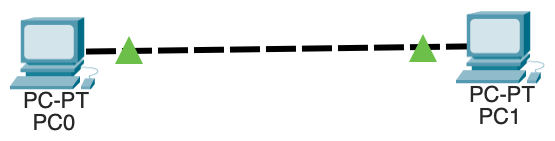
\includegraphics[width=0.75\textwidth]{images/q1_topology.png}
    \caption{Question 1: Direct back-to-back host topology connected with a Copper Cross-Over cable.}
    \label{fig:q1_top}
\end{figure}

\begin{figure}[H]
    \centering
    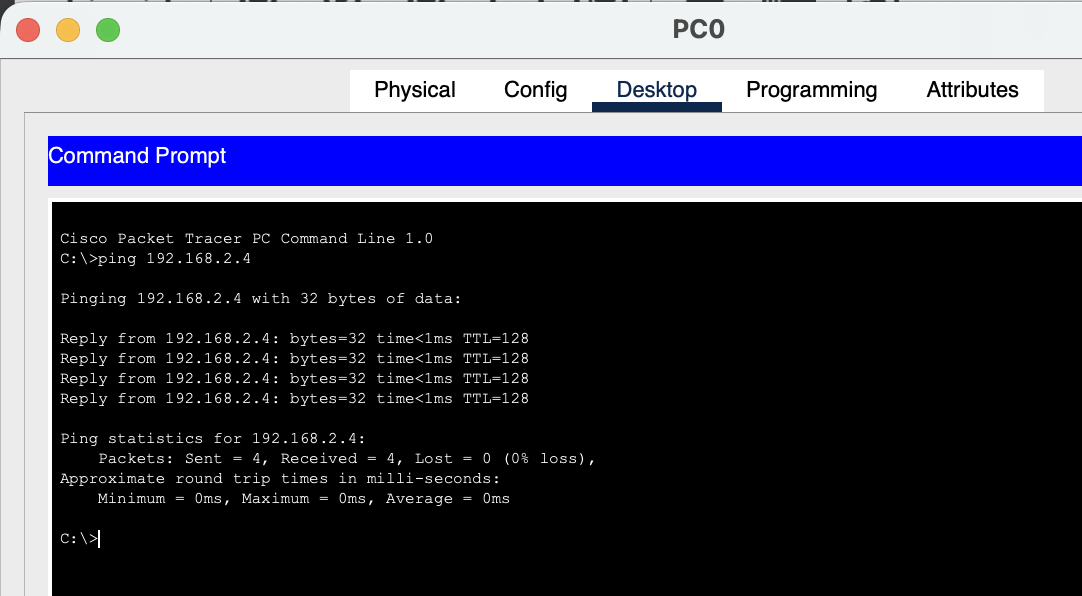
\includegraphics[width=0.88\textwidth]{images/q1_ping.png}
    \caption{Question 1: ICMP ping execution on PC0 targeting PC1 (192.168.2.4) showing 0\% loss and $<1\,\text{ms}$ RTT.}
    \label{fig:q1_ping}
\end{figure}

\textbf{Inference:} Direct communication between two computing systems is achieved without intermediate hubs, switches, or routers when physical pinouts match and hosts reside on the same IP subnet.

\newpage

% ==================== SECTION 3: QUESTION 2 ====================
\section{Question 2: Hub-Based Local Area Network (LAN-A)}

\subsection{Problem Statement \& Mechanism of Operation}
Construct a 3-host local area network named \textbf{LAN-A} using a central hub (\texttt{Hub-PT}) and verify pairwise connectivity between all hosts.

A network Hub operates strictly at Layer 1. When an electrical signal enters any port, the repeater regenerates it onto all other ports:
\begin{itemize}
    \item \textbf{Single Collision Domain:} All three hosts share one physical transmission channel. Simultaneous transmissions cause physical collisions requiring CSMA/CD backoff.
    \item \textbf{Half-Duplex:} Hosts cannot transmit and receive simultaneously.
    \item \textbf{Shared Medium:} Every packet is delivered to all connected stations, regardless of destination MAC.
\end{itemize}

\subsection{Addressing Scheme}
\begin{itemize}
    \item \texttt{LAN-A-PC0}: \texttt{192.168.2.1} / \texttt{255.255.255.0}
    \item \texttt{LAN-A-PC1}: \texttt{192.168.2.2} / \texttt{255.255.255.0}
    \item \texttt{LAN-A-PC2}: \texttt{192.168.2.3} / \texttt{255.255.255.0}
\end{itemize}

\begin{figure}[H]
    \centering
    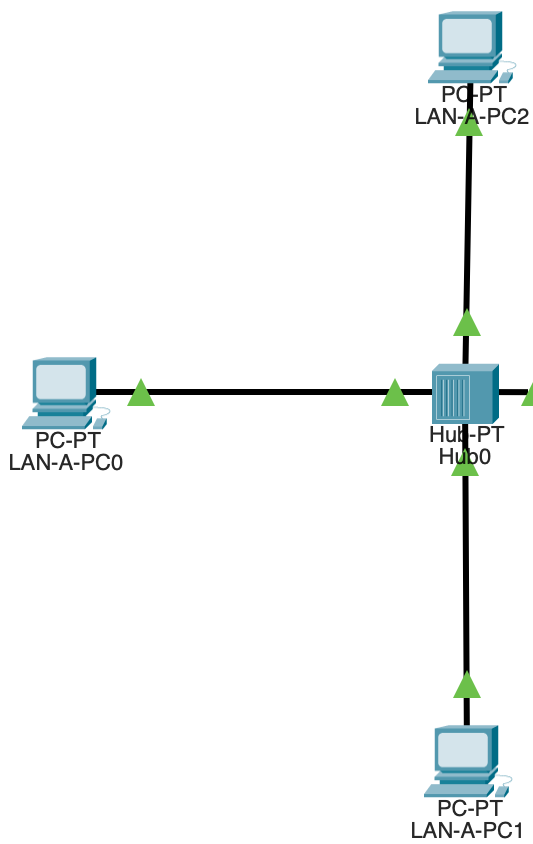
\includegraphics[width=0.55\textwidth]{images/q2_topology.png}
    \caption{Question 2: LAN-A hub-based star topology with 3 workstations.}
    \label{fig:q2_top}
\end{figure}

\begin{figure}[H]
    \centering
    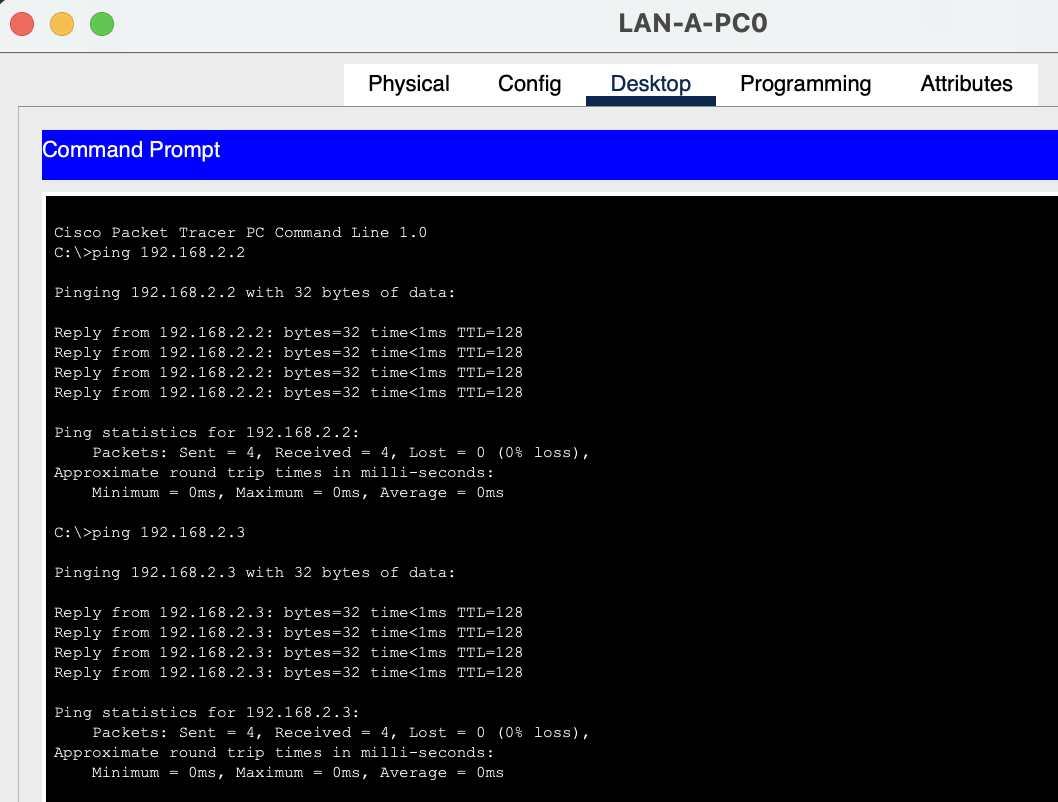
\includegraphics[width=0.88\textwidth]{images/q2_ping_pc0.png}
    \caption{Question 2: Pairwise ping execution on PC0 targeting PC1 (192.168.2.2) and PC2 (192.168.2.3).}
    \label{fig:q2_p0}
\end{figure}

\newpage

\begin{figure}[H]
    \centering
    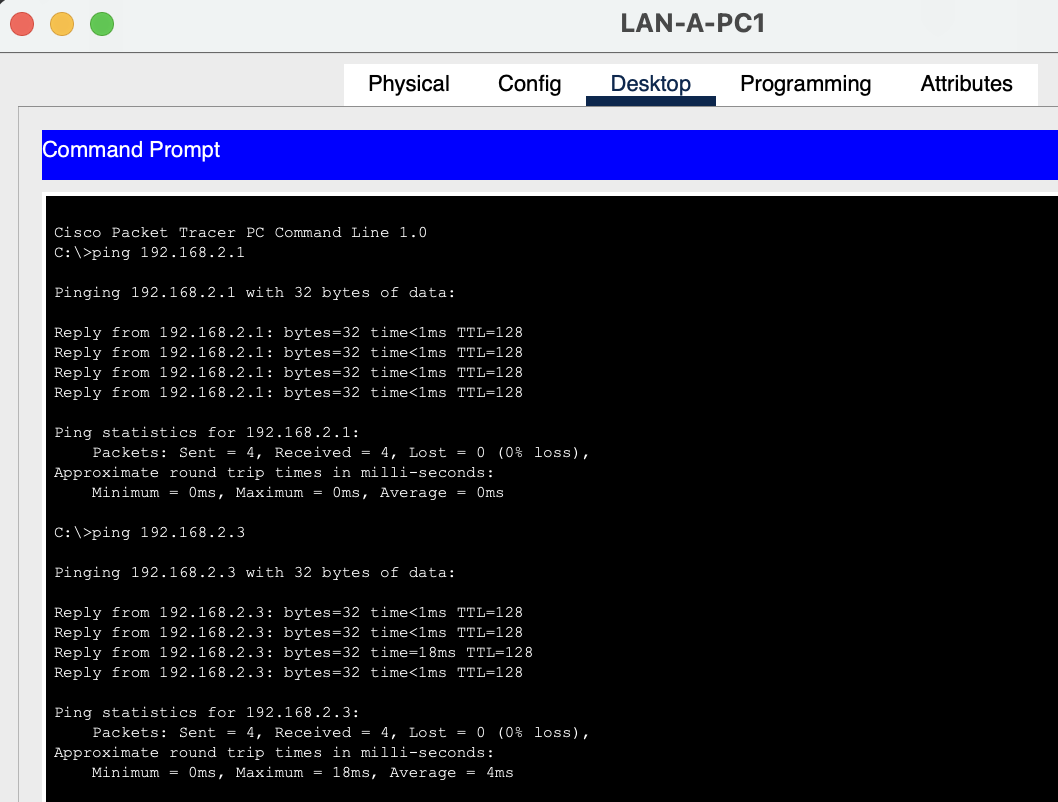
\includegraphics[width=0.88\textwidth]{images/q2_ping_pc1.png}
    \caption{Question 2: Pairwise ping execution on PC1 targeting PC0 (192.168.2.1) and PC2 (192.168.2.3).}
    \label{fig:q2_p1}
\end{figure}

\begin{figure}[H]
    \centering
    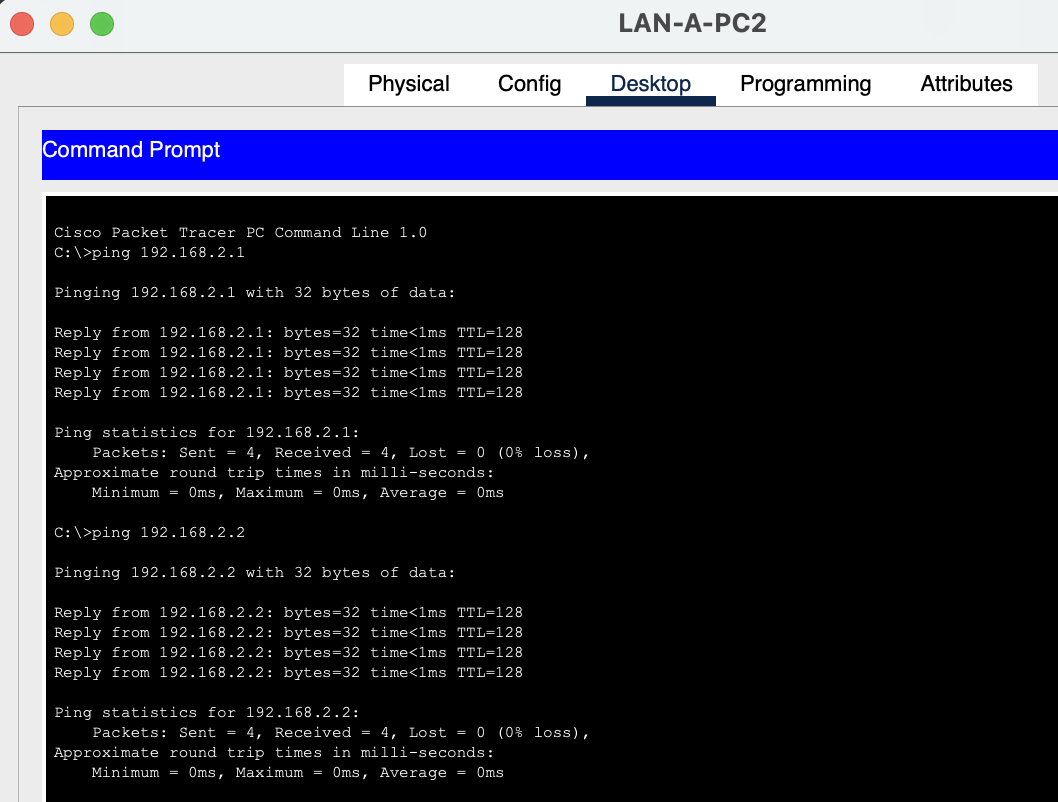
\includegraphics[width=0.88\textwidth]{images/q2_ping_pc2.png}
    \caption{Question 2: Pairwise ping execution on PC2 targeting PC0 (192.168.2.1) and PC1 (192.168.2.2).}
    \label{fig:q2_p2}
\end{figure}

\textbf{Inference:} All pairwise communications succeeded with 0\% packet loss. However, every transmission occupied the shared bandwidth of all connected links simultaneously.

\newpage

% ==================== SECTION 4: QUESTION 3 ====================
\section{Question 3: Switch-Based LAN (LAN-B) \& CAM/ARP Dynamics}

\subsection{Problem Statement \& Theoretical Framework}
Construct **LAN-B** using a Cisco Catalyst 2960 Layer-2 switch. Record host **ARP Tables** and the switch **MAC Address Table (CAM Table)** both \emph{before} and \emph{after} generating traffic.

\begin{itemize}
    \item \textbf{Micro-segmentation:} Each switch port forms an isolated collision domain, operating in full-duplex.
    \item \textbf{CAM Learning Algorithm:} The switch inspects the source MAC of incoming frames and maps it to the ingress port. If the destination MAC is known, it forwards unicast frames directly to the mapped port; otherwise, it floods the frame.
    \item \textbf{ARP (RFC 826):} Hosts resolve 32-bit IPv4 addresses to 48-bit MAC addresses via broadcast requests and unicast replies.
\end{itemize}

\subsection{Pre-Communication Baseline}
Prior to generating any network traffic, the tables were inspected:
\begin{itemize}
    \item \texttt{arp -a} on \texttt{LAN-B-PC1}: \texttt{No ARP Entries Found}.
    \item \texttt{show mac address-table} on the switch: Empty dynamic table.
\end{itemize}

\begin{figure}[H]
    \centering
    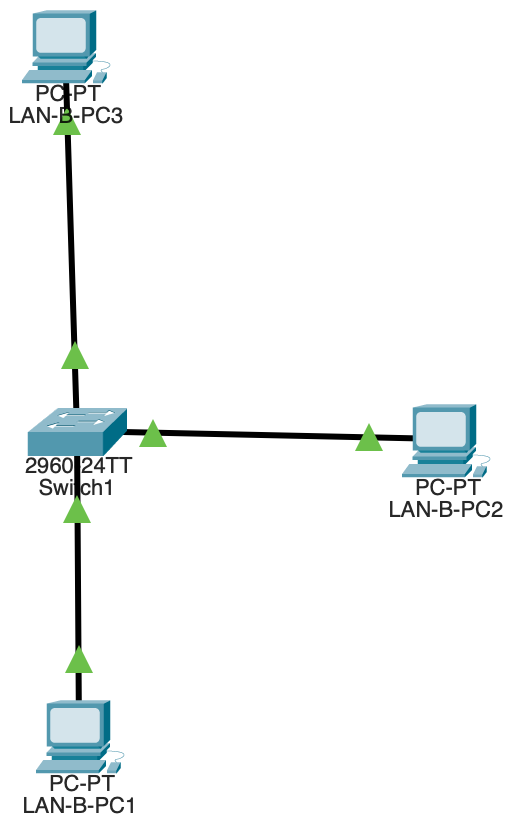
\includegraphics[width=0.55\textwidth]{images/q3_topology.png}
    \caption{Question 3: LAN-B switch topology using a Cisco Catalyst 2960 switch.}
    \label{fig:q3_top}
\end{figure}

\begin{figure}[H]
    \centering
    \begin{subfigure}[b]{0.49\textwidth}
        \centering
        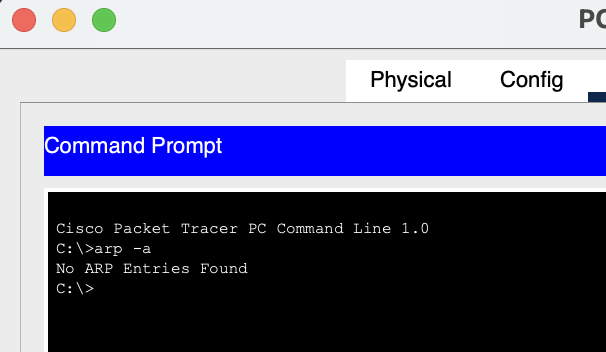
\includegraphics[width=\textwidth]{images/q3_arp_initial.png}
        \caption{Pre-ping host ARP cache: empty.}
        \label{fig:q3_arp_init}
    \end{subfigure}
    \hfill
    \begin{subfigure}[b]{0.49\textwidth}
        \centering
        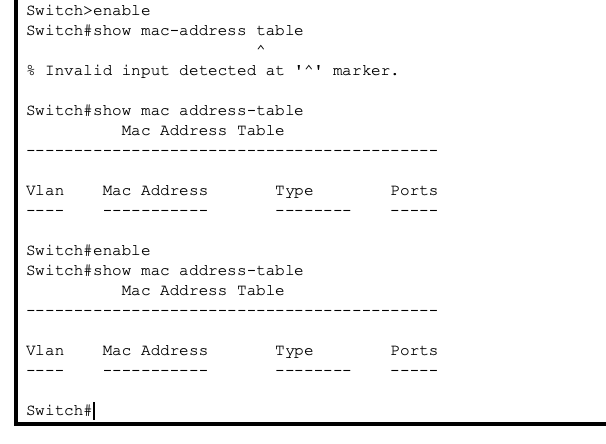
\includegraphics[width=\textwidth]{images/q3_mac_table_initial.png}
        \caption{Pre-ping switch CAM table: empty.}
        \label{fig:q3_cam_init}
    \end{subfigure}
    \caption{Question 3: Pre-communication baseline showing unpopulated state tables.}
    \label{fig:q3_init_tables}
\end{figure}

\newpage

\subsection{Traffic Generation \& Post-Communication State Evolution}
Workstation \texttt{LAN-B-PC1} executed pings targeting \texttt{PC2} (\texttt{192.168.2.2}) and \texttt{PC3} (\texttt{192.168.2.3}).

\begin{figure}[H]
    \centering
    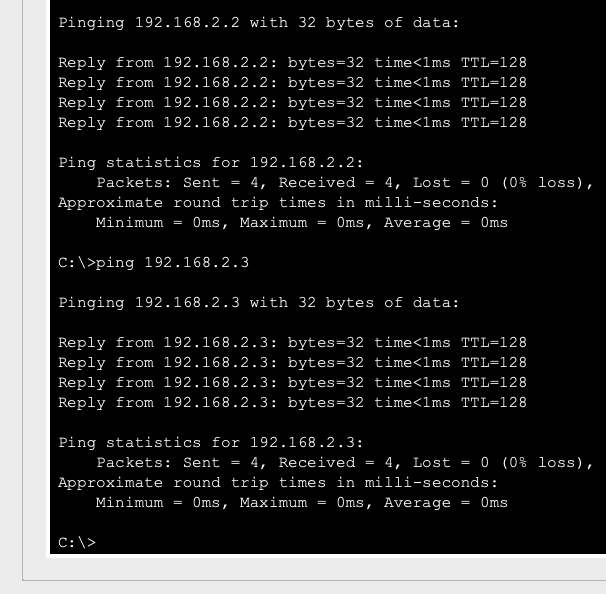
\includegraphics[width=0.82\textwidth]{images/q3_ping.png}
    \caption{Question 3: ICMP ping sequence from LAN-B-PC1 to PC2 (192.168.2.2) and PC3 (192.168.2.3).}
    \label{fig:q3_ping}
\end{figure}

\begin{figure}[H]
    \centering
    \begin{subfigure}[b]{0.49\textwidth}
        \centering
        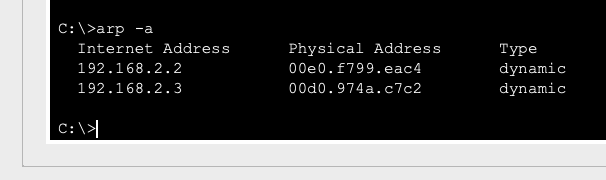
\includegraphics[width=\textwidth]{images/q3_arp_after.png}
        \caption{Post-ping host ARP cache populated dynamically.}
        \label{fig:q3_arp_aft}
    \end{subfigure}
    \hfill
    \begin{subfigure}[b]{0.49\textwidth}
        \centering
        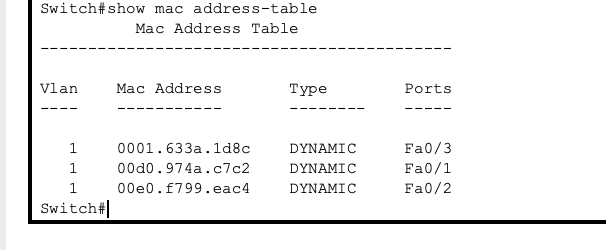
\includegraphics[width=\textwidth]{images/q3_mac_table_after.png}
        \caption{Post-ping switch CAM table showing learned ports.}
        \label{fig:q3_cam_aft}
    \end{subfigure}
    \caption{Question 3: Post-communication tables showing dynamic ARP and CAM resolution.}
    \label{fig:q3_aft_tables}
\end{figure}

\textbf{Inference:}
\begin{enumerate}
    \item \texttt{PC1}'s ARP table dynamically resolved \texttt{192.168.2.2} $\rightarrow$ \texttt{00e0.f799.eac4} and \texttt{192.168.2.3} $\rightarrow$ \texttt{00d0.974a.c7c2}.
    \item The switch CAM table dynamically learned ports \texttt{Fa0/1}, \texttt{Fa0/2}, and \texttt{Fa0/3} for the respective MAC addresses, eliminating subsequent unicast flooding.
\end{enumerate}

\newpage

% ==================== SECTION 5: QUESTION 4 ====================
\section{Question 4: Inter-LAN Bridging (Hub to Switch Interconnection)}

\subsection{Problem Statement \& Subnet Boundary Principle}
Connect LAN-A (Hub) and LAN-B (Switch) using a Copper Cross-Over cable, test connectivity across LANs, and observe ARP and switch CAM table changes.

\textbf{Subnet Boundary Principle:} A hub and a switch operate at Layer 1 and Layer 2. If LAN-A and LAN-B belonged to different IP subnets (e.g. \texttt{192.168.2.0/24} and \texttt{192.168.3.0/24}), hosts would drop frames because they look for an absent Layer-3 default gateway. To enable flat Layer-2 bridging across the crossover cable without a router, all six workstations were assigned IP addresses within the unified subnet \texttt{192.168.2.0/24}.

\begin{figure}[H]
    \centering
    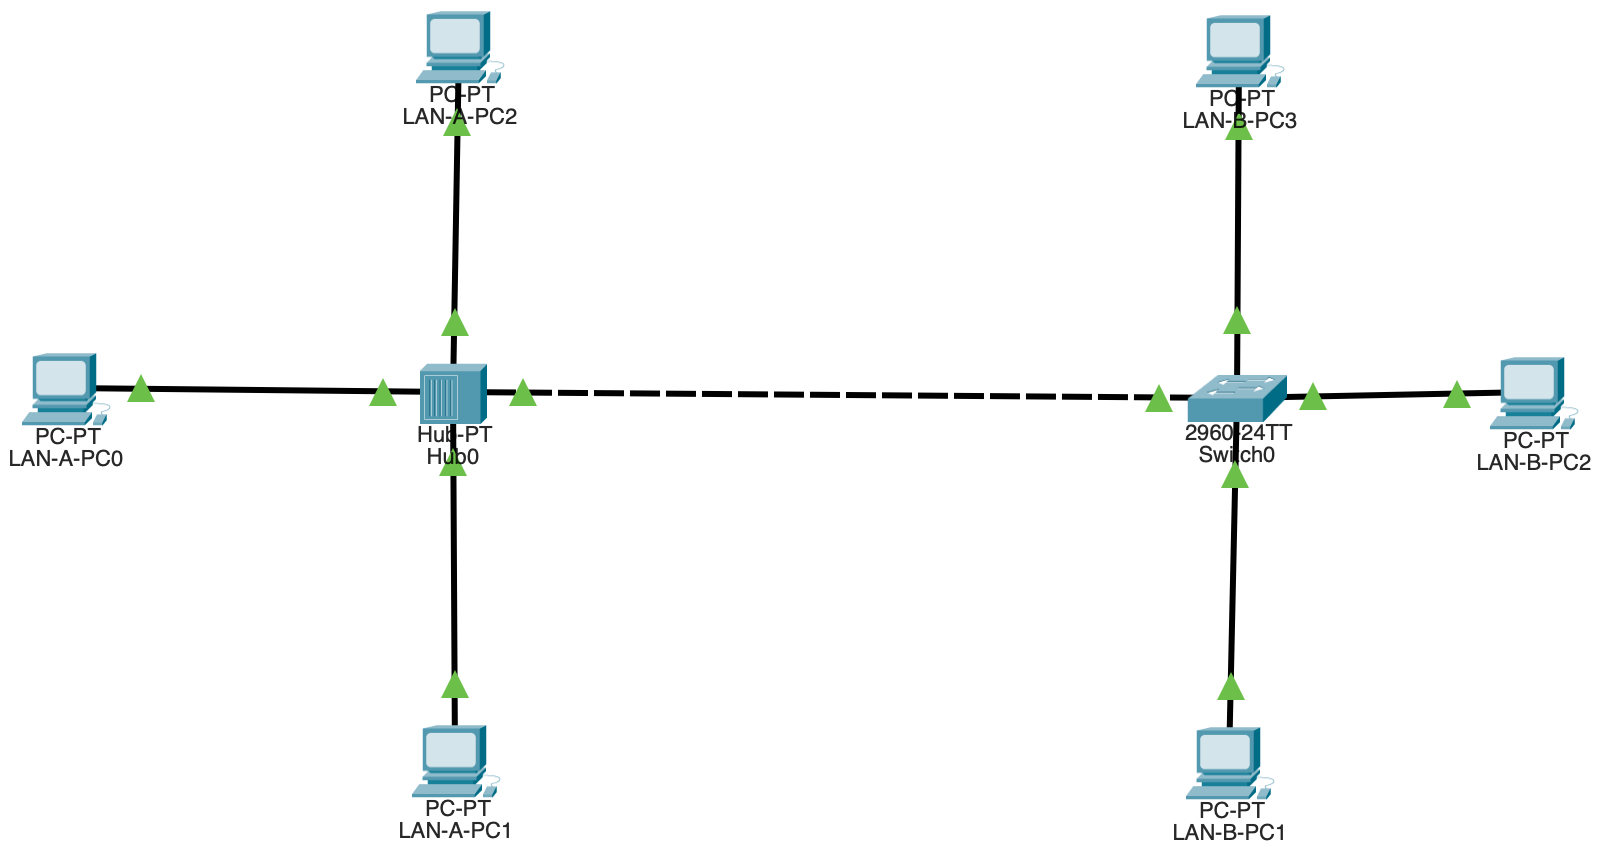
\includegraphics[width=0.88\textwidth]{images/q4_topology.png}
    \caption{Question 4: Interconnected topology linking Hub0 to Switch0 via a crossover cable.}
    \label{fig:q4_top}
\end{figure}

\begin{figure}[H]
    \centering
    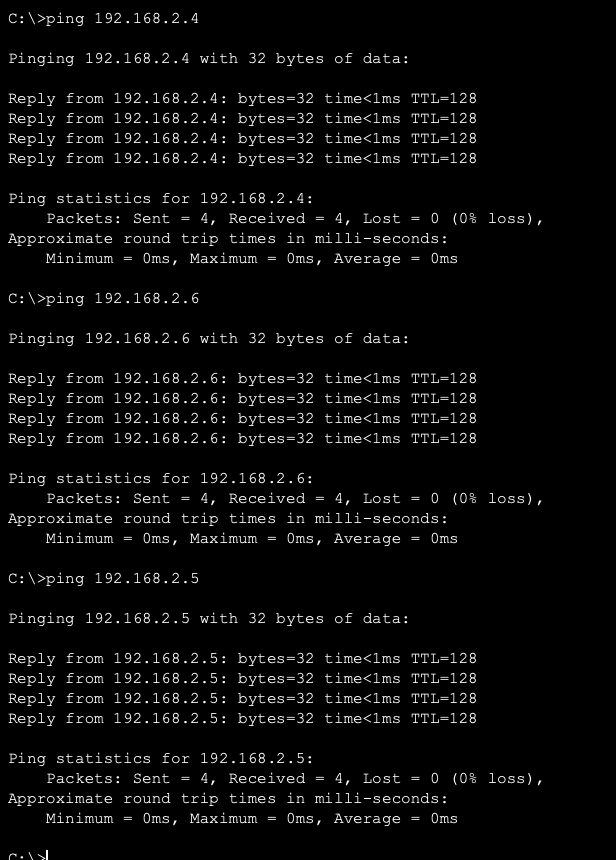
\includegraphics[width=0.80\textwidth]{images/q4_ping.png}
    \caption{Question 4: Cross-LAN ping execution from LAN-A-PC1 to LAN-B hosts (192.168.2.4, .2.6, .2.5).}
    \label{fig:q4_ping}
\end{figure}

\newpage

\subsection{Uplink Port Multi-MAC Address Learning}
Figure~\ref{fig:q4_tables} displays the post-ping ARP table of \texttt{LAN-A-PC1} and the switch CAM table.

\begin{figure}[H]
    \centering
    \begin{subfigure}[b]{0.49\textwidth}
        \centering
        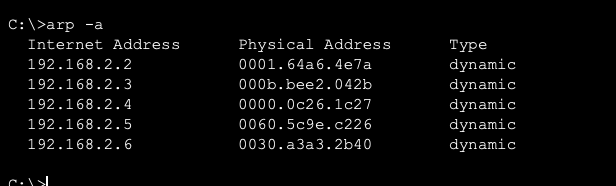
\includegraphics[width=\textwidth]{images/q4_arp_after.png}
        \caption{LAN-A-PC1 ARP table containing all 5 nodes.}
        \label{fig:q4_arp}
    \end{subfigure}
    \hfill
    \begin{subfigure}[b]{0.49\textwidth}
        \centering
        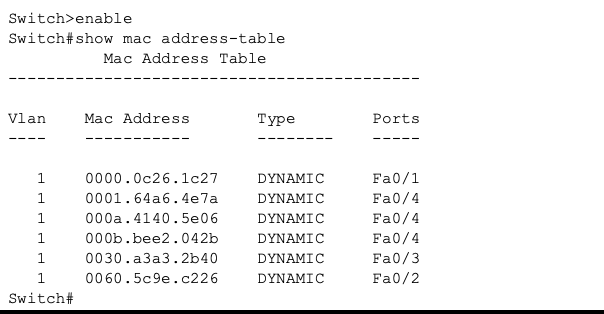
\includegraphics[width=\textwidth]{images/q4_mac_table_after.png}
        \caption{Switch CAM table showing multi-MAC on Fa0/4.}
        \label{fig:q4_cam}
    \end{subfigure}
    \caption{Question 4: State tables showing multi-MAC learning on the hub uplink port.}
    \label{fig:q4_tables}
\end{figure}

\textbf{Key Observation:} On the switch, ports \texttt{Fa0/1}, \texttt{Fa0/2}, and \texttt{Fa0/3} map to one MAC address each. Port \texttt{Fa0/4} (the link to the hub) dynamically learned \textbf{three MAC addresses} (\texttt{0001.64a6.4e7a}, \texttt{000a.4140.5e06}, \texttt{000b.bee2.042b}). This demonstrates that an uplink port connected to a shared or bridged segment legitimately associates multiple MAC addresses with a single physical switch port.

\newpage

% ==================== SECTION 6: QUESTION 5 ====================
\section{Question 5: Multi-Router Inter-Network Routing over Serial WAN}

\subsection{Architecture \& Interface Configuration}
Experiment 5 interconnects two enterprise campus LANs across a synchronous serial WAN link:
\begin{itemize}
    \item \textbf{JU-Main LAN:} \texttt{192.168.148.0/24}, Gateway \texttt{192.168.148.1} (\texttt{Gig0/0} on \texttt{JU-Main-Router}).
    \item \textbf{JU-SL LAN:} \texttt{192.168.149.0/24}, Gateway \texttt{192.168.149.1} (\texttt{Gig0/0} on \texttt{JU-SL-Router}).
    \item \textbf{WAN Serial Link:} \texttt{192.168.150.0/24} over \texttt{WIC-2T} interfaces. \texttt{JU-Main-Router} acts as DCE (\texttt{clock rate 64000}).
\end{itemize}

\begin{lstlisting}[caption={Static route configurations on the routers.}]
! On JU-Main-Router:
ip route 192.168.149.0 255.255.255.0 192.168.150.2

! On JU-SL-Router:
ip route 192.168.148.0 255.255.255.0 192.168.150.1
\end{lstlisting}

\begin{figure}[H]
    \centering
    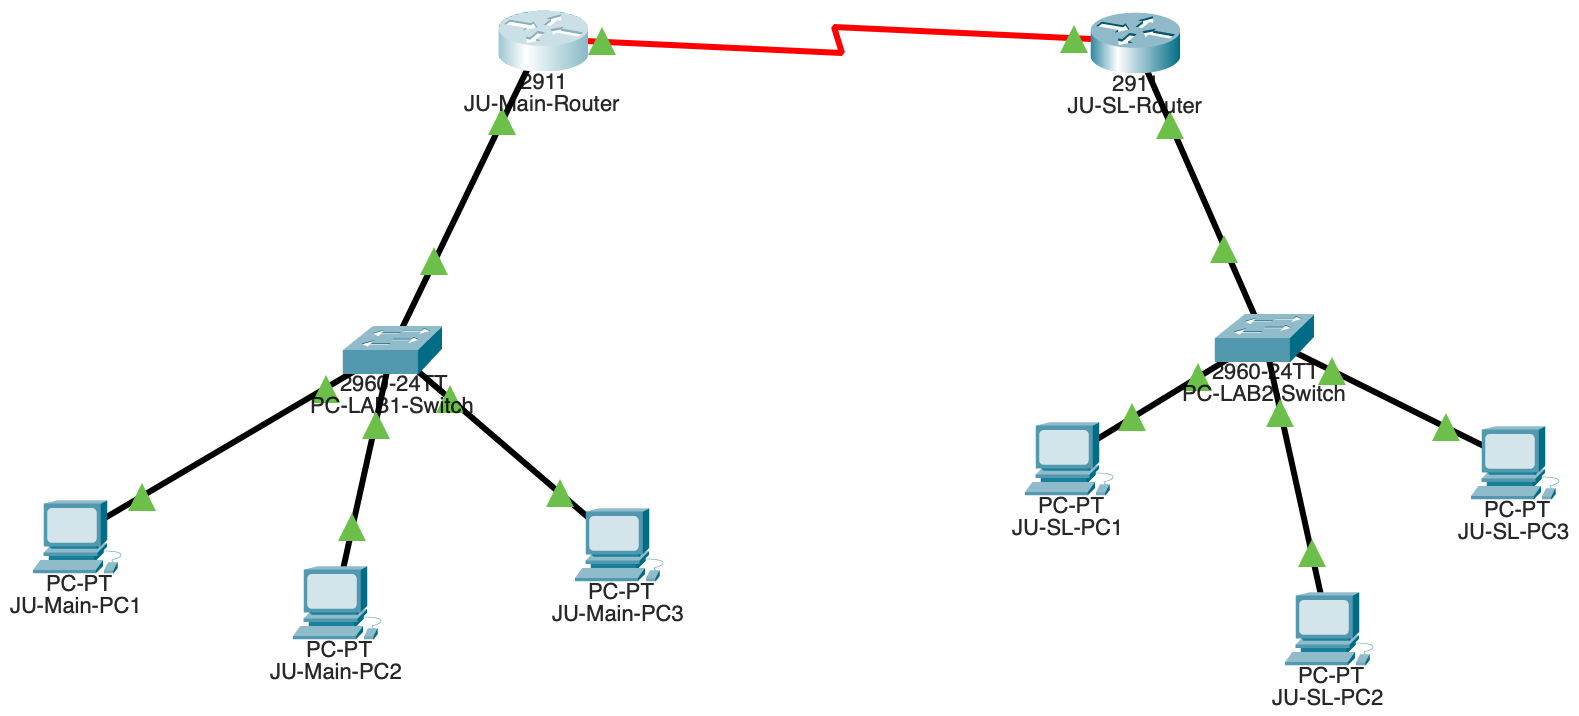
\includegraphics[width=0.92\textwidth]{images/q5_topology.png}
    \caption{Question 5: Enterprise multi-router topology interconnecting JU-Main and JU-SL across a serial WAN.}
    \label{fig:q5_top}
\end{figure}

\begin{figure}[H]
    \centering
    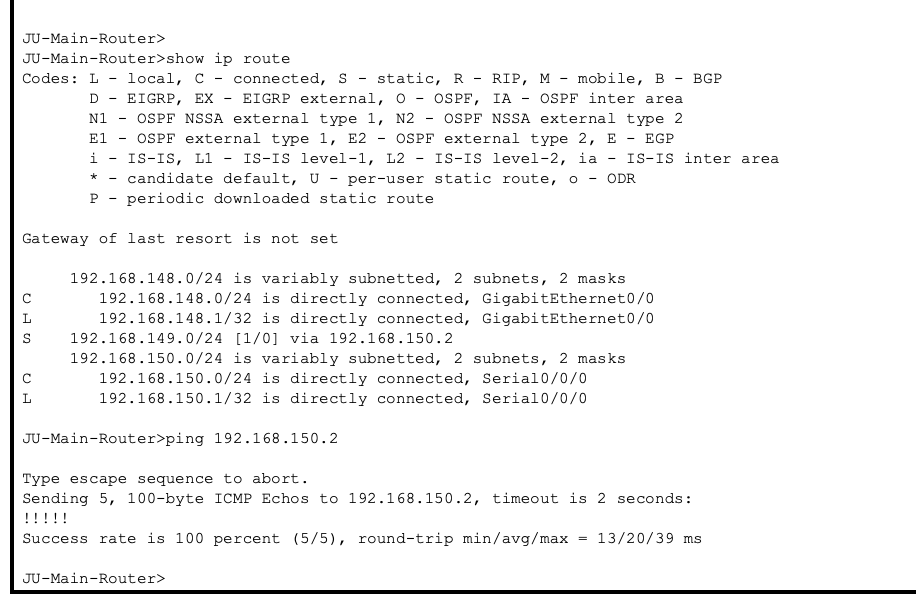
\includegraphics[width=0.85\textwidth]{images/q5_routing_tables.png}
    \caption{Question 5: Cisco IOS routing tables on JU-Main-Router and JU-SL-Router verifying static routes.}
    \label{fig:q5_routes}
\end{figure}

\newpage

\begin{figure}[H]
    \centering
    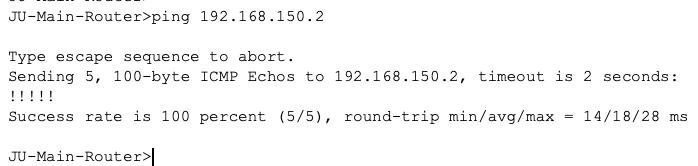
\includegraphics[width=0.85\textwidth]{images/q5_wan_ping.png}
    \caption{Question 5: Point-to-point WAN ping test across serial link (100\% success rate).}
    \label{fig:q5_wan}
\end{figure}

\begin{figure}[H]
    \centering
    \begin{subfigure}[b]{0.49\textwidth}
        \centering
        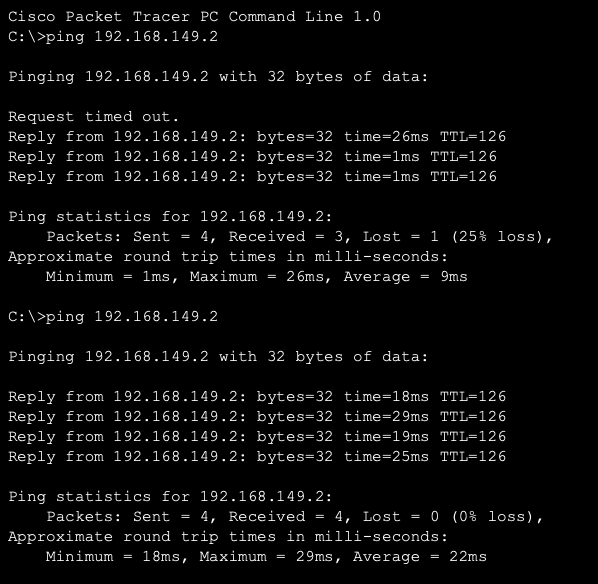
\includegraphics[width=\textwidth]{images/q5_ping_main_to_sl.png}
        \caption{JU-Main-PC1 pinging remote JU-SL-PC1.}
        \label{fig:q5_p_main}
    \end{subfigure}
    \hfill
    \begin{subfigure}[b]{0.49\textwidth}
        \centering
        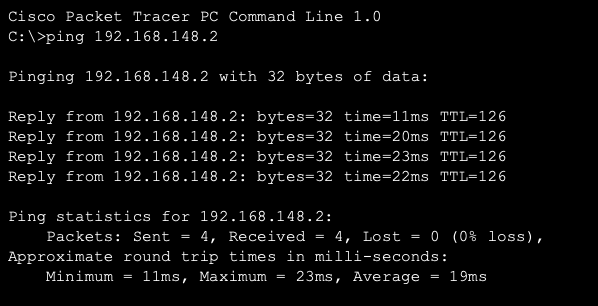
\includegraphics[width=\textwidth]{images/q5_ping_sl_to_main.png}
        \caption{JU-SL-PC1 pinging remote JU-Main-PC1.}
        \label{fig:q5_p_sl}
    \end{subfigure}
    \caption{Question 5: Bidirectional ping verification between workstations across the routed WAN.}
    \label{fig:q5_pc_pings}
\end{figure}

\textbf{Analysis of Initial Packet Timeout:}
In Figure~\ref{fig:q5_p_main}, the first ping packet reported \texttt{Request timed out}. This is an expected artifact of a double ARP resolution: \texttt{JU-Main-PC1} had to resolve its default gateway, and \texttt{JU-SL-Router} had to resolve the destination host's MAC address. Once cached, subsequent pings achieved 100\% success with $\text{TTL} = 126$ ($128 - 2\text{ router hops}$).

\newpage

% ==================== SECTION 7: QUESTION 6 ====================
\section{Question 6: Dynamic Host Configuration Protocol (DHCP)}

\subsection{Problem Statement \& DORA Protocol Exchange}
Deploy dedicated DHCP servers in each LAN (\texttt{JU-Main} and \texttt{JU-SL}) and configure all workstations to obtain IP addresses and default gateways dynamically via the four-stage DORA exchange (Discover, Offer, Request, Acknowledge).

\begin{itemize}
    \item \texttt{JU-Main-DHCP-Server}: Static IP \texttt{192.168.148.10}, Gateway \texttt{192.168.148.1}, Pool \texttt{192.168.148.100+}.
    \item \texttt{JU-SL-DHCP-Server}: Static IP \texttt{192.168.149.10}, Gateway \texttt{192.168.149.1}, Pool \texttt{192.168.149.100+}.
\end{itemize}

\begin{figure}[H]
    \centering
    \begin{subfigure}[b]{0.49\textwidth}
        \centering
        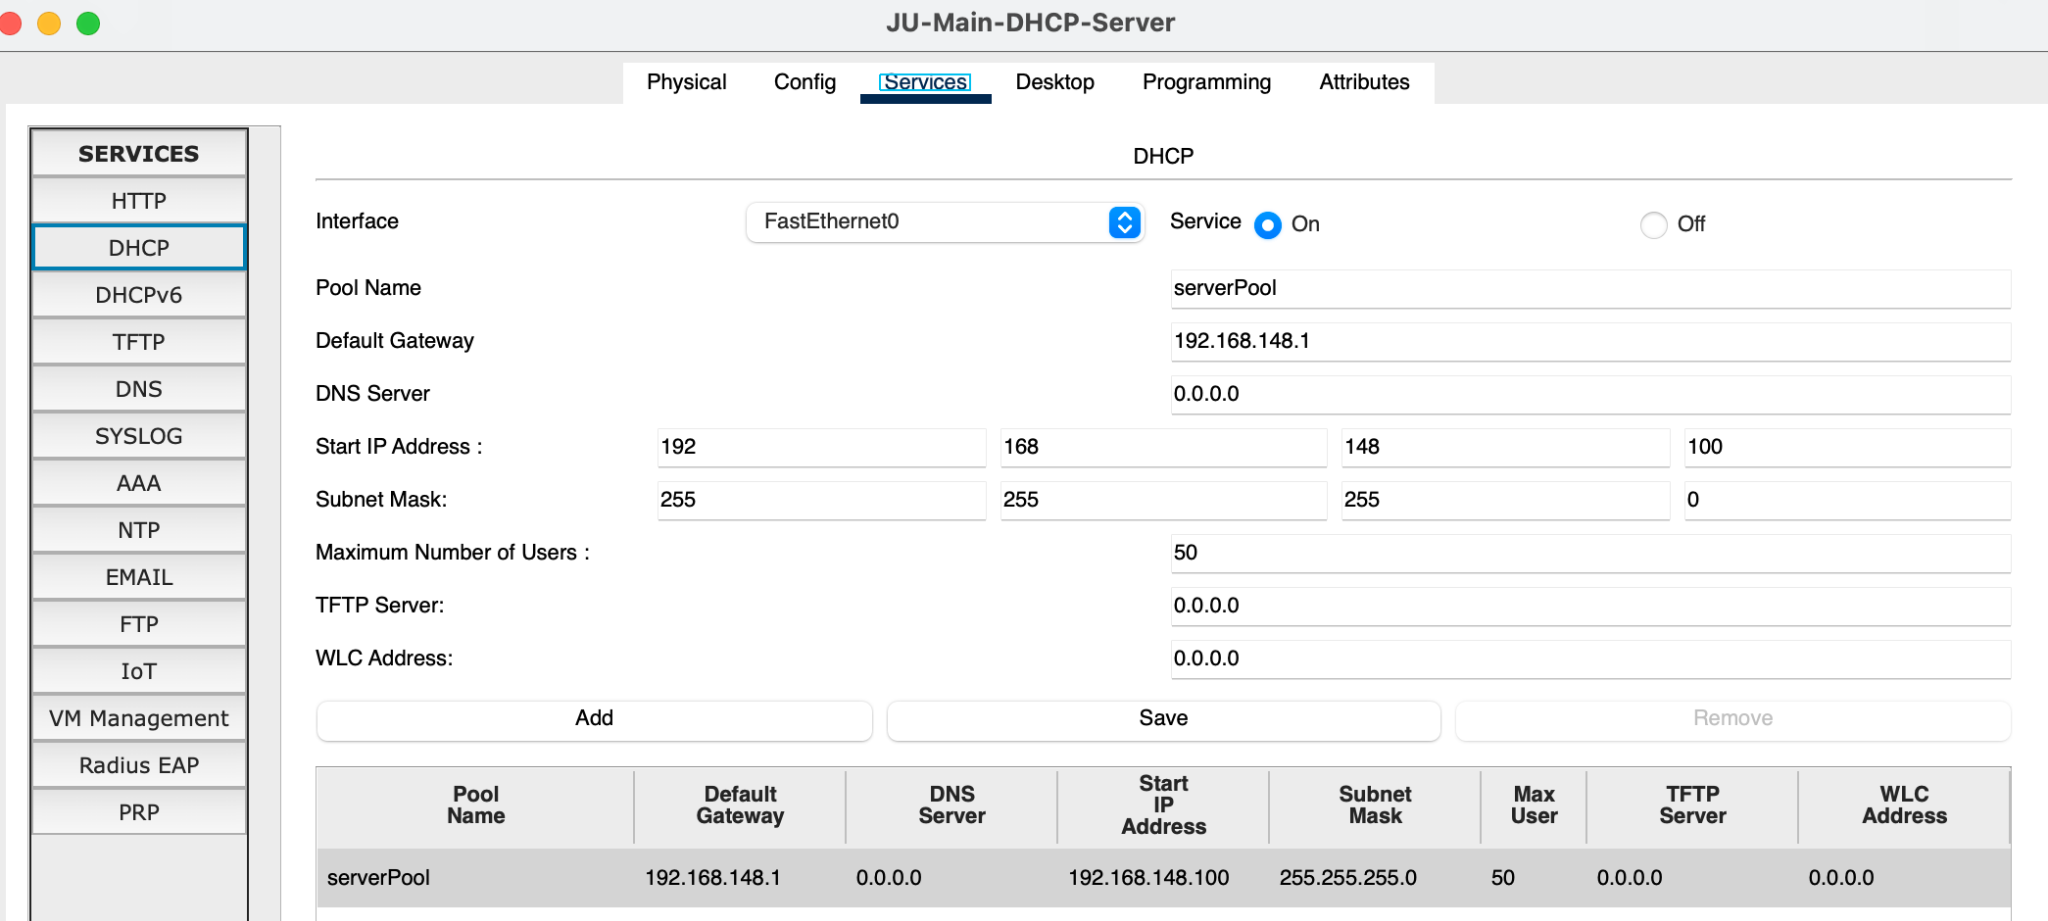
\includegraphics[width=\textwidth]{images/q6_dhcp_server_main.png}
        \caption{JU-Main DHCP service configuration.}
        \label{fig:q6_srv_main}
    \end{subfigure}
    \hfill
    \begin{subfigure}[b]{0.49\textwidth}
        \centering
        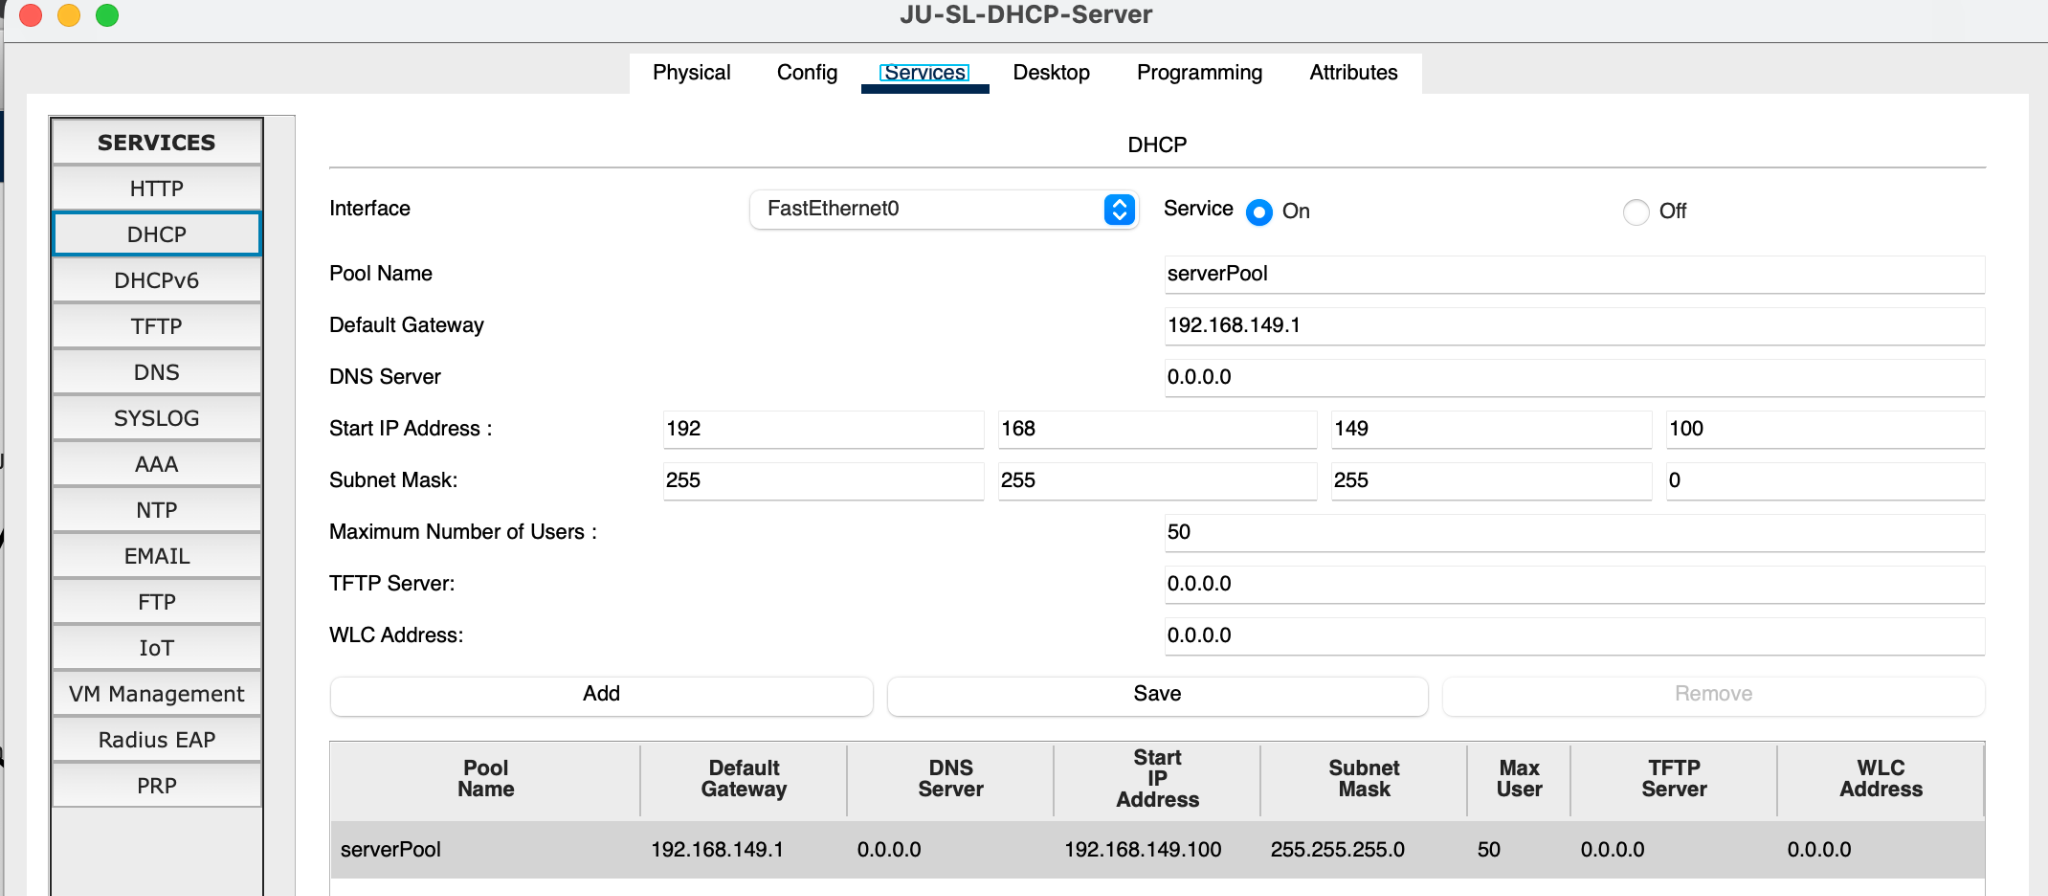
\includegraphics[width=\textwidth]{images/q6_dhcp_server_sl.png}
        \caption{JU-SL DHCP service configuration.}
        \label{fig:q6_srv_sl}
    \end{subfigure}
    \caption{Question 6: DHCP service pool definitions with gateway and IP ranges.}
    \label{fig:q6_srv_config}
\end{figure}

\begin{figure}[H]
    \centering
    \begin{subfigure}[b]{0.49\textwidth}
        \centering
        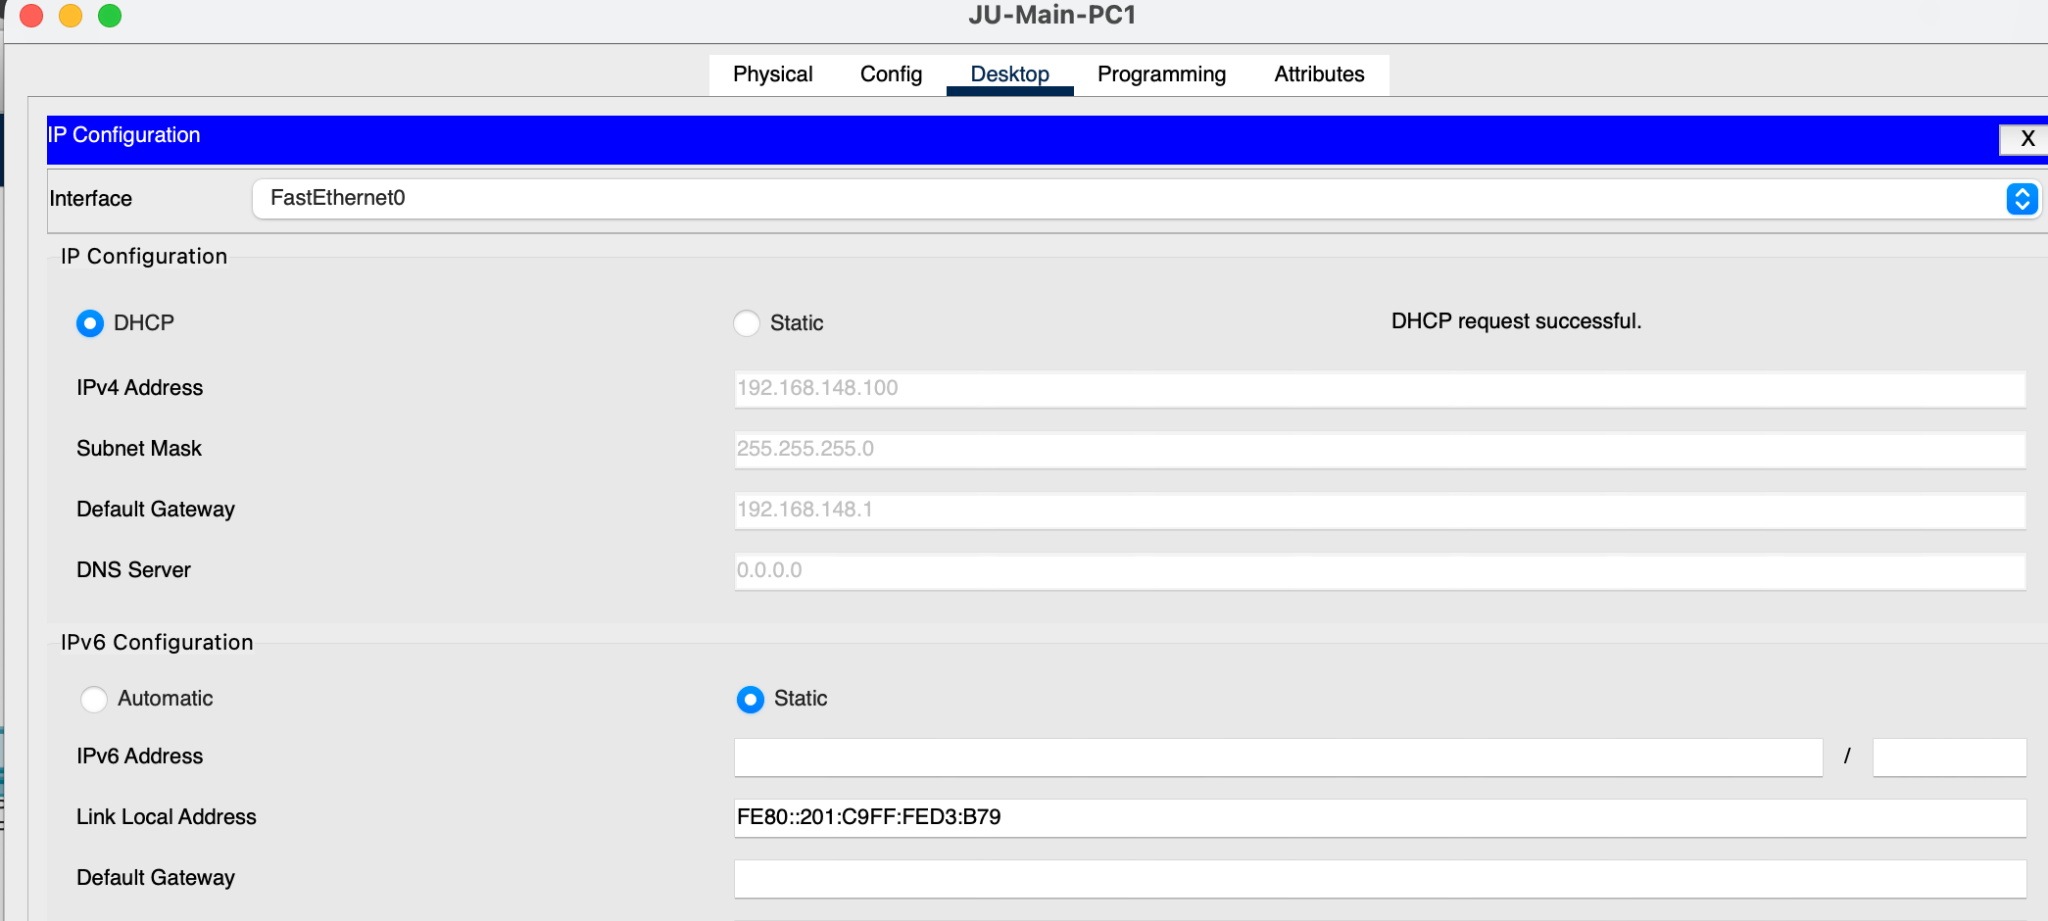
\includegraphics[width=\textwidth]{images/q6_pc_dhcp_main.png}
        \caption{JU-Main-PC1 successful DHCP lease.}
        \label{fig:q6_pc_main}
    \end{subfigure}
    \hfill
    \begin{subfigure}[b]{0.49\textwidth}
        \centering
        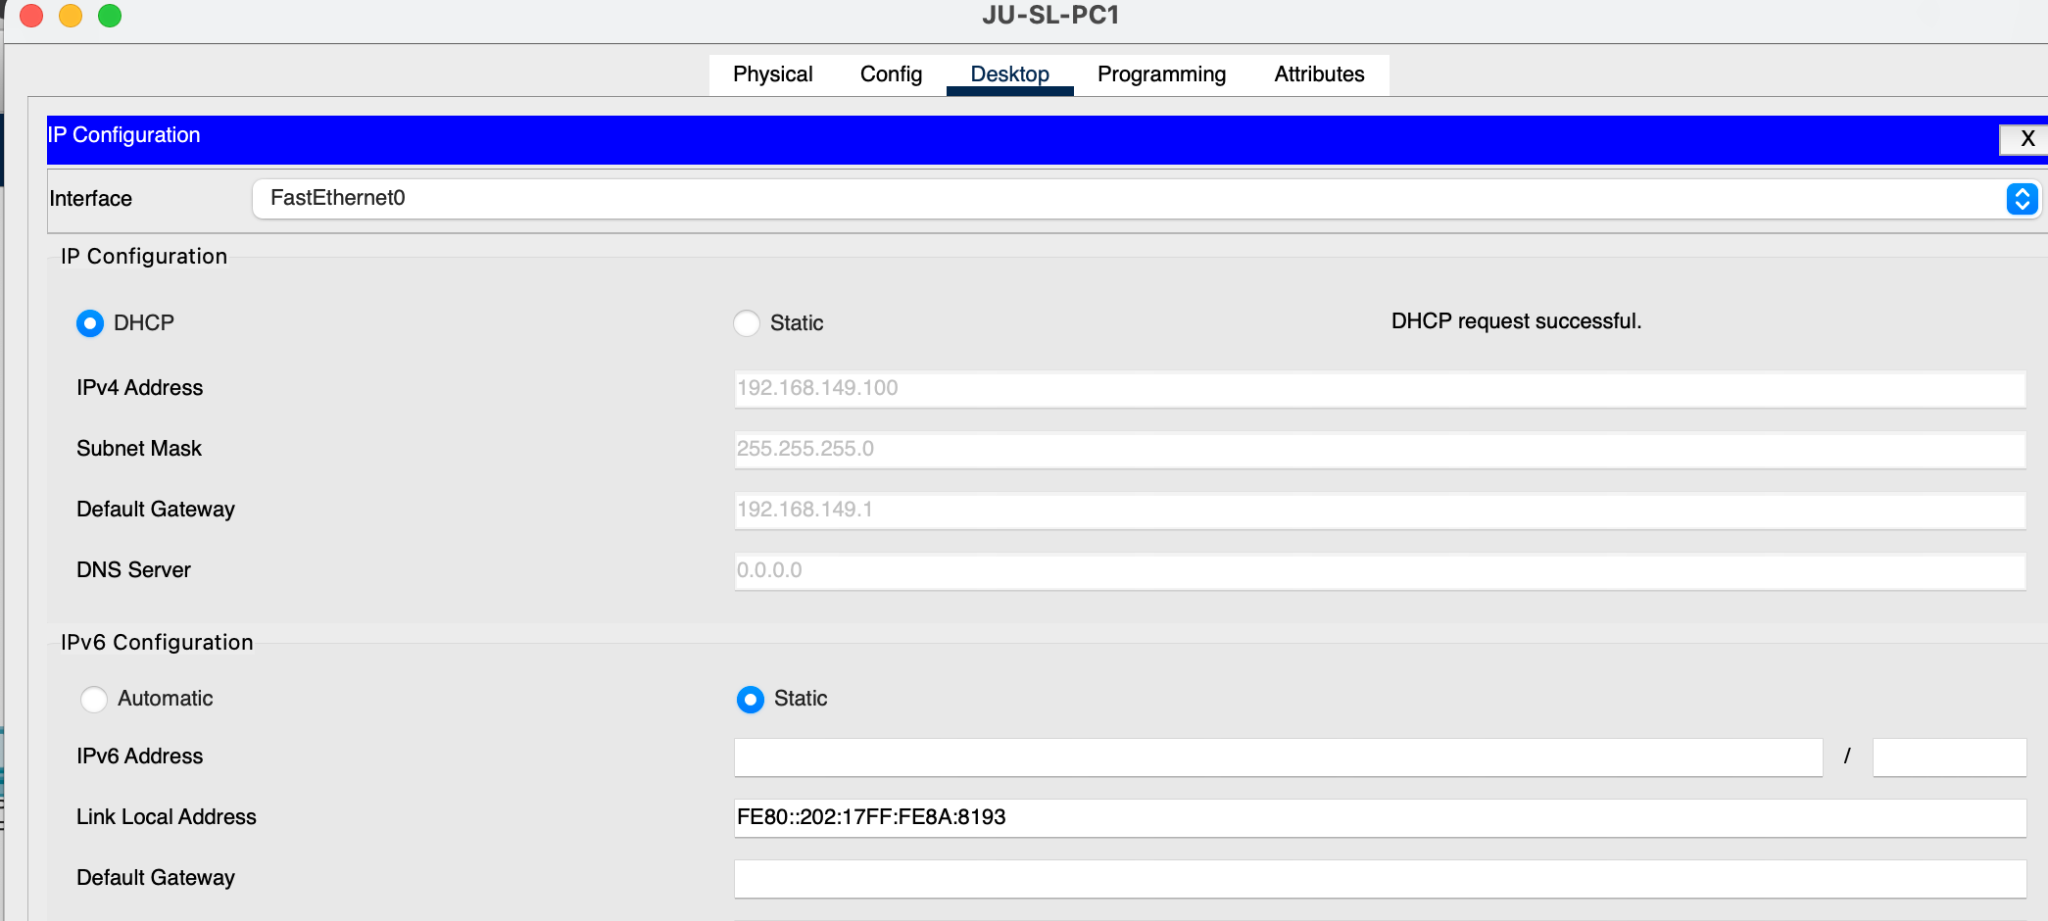
\includegraphics[width=\textwidth]{images/q6_pc_dhcp_sl.png}
        \caption{JU-SL-PC1 successful DHCP lease.}
        \label{fig:q6_pc_sl}
    \end{subfigure}
    \caption{Question 6: Workstation IP panels displaying "DHCP request successful!".}
    \label{fig:q6_pc_dhcp}
\end{figure}

\newpage

\begin{figure}[H]
    \centering
    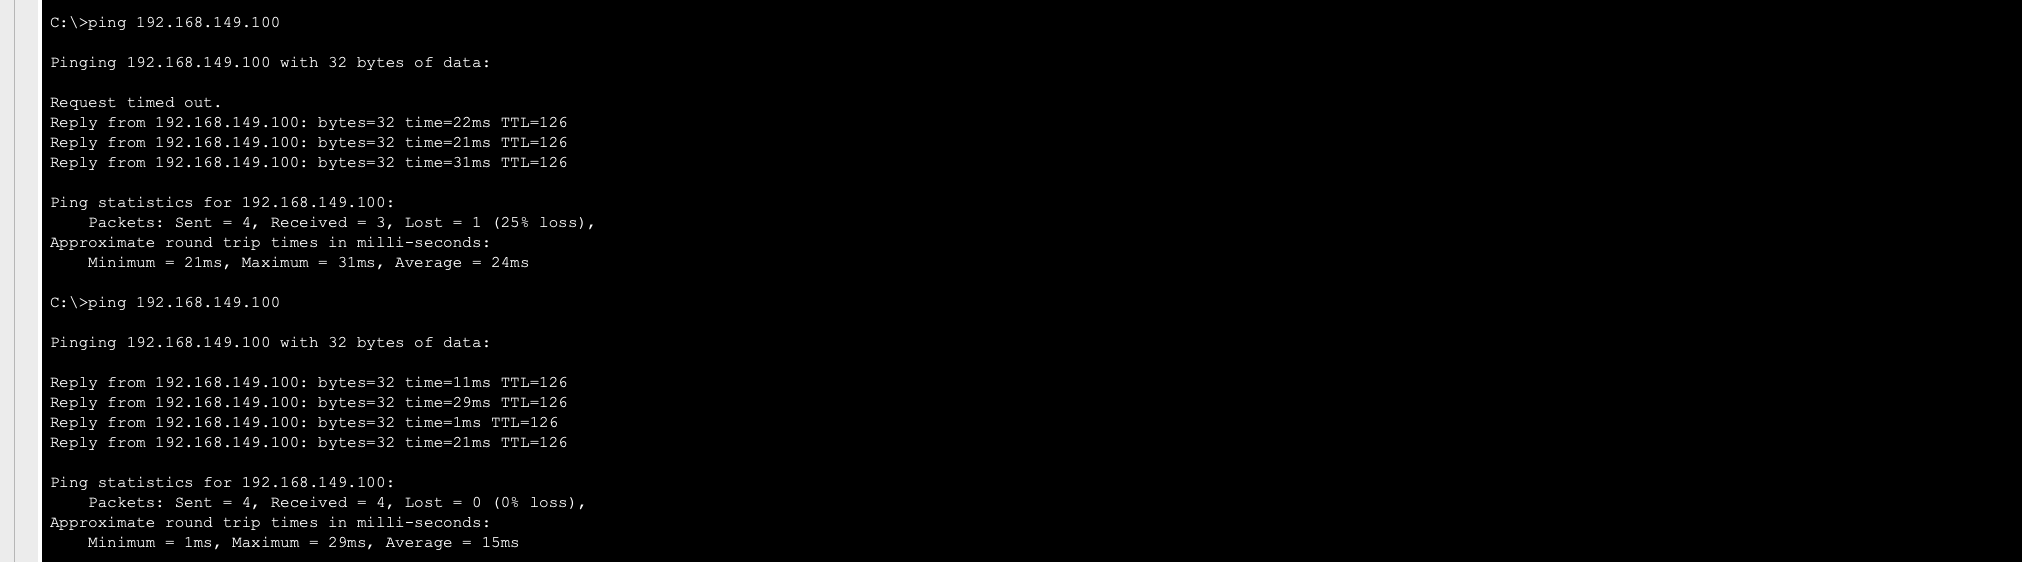
\includegraphics[width=0.88\textwidth]{images/q6_ping_dhcp.png}
    \caption{Question 6: End-to-end ping verification between DHCP-configured workstations across the routed WAN.}
    \label{fig:q6_ping}
\end{figure}

\textbf{Inference:} Dynamic leasing completed successfully, and end-to-end reachability was verified between hosts across the routed WAN at dynamically assigned IP \texttt{192.168.149.100}.

\newpage

% ==================== SECTION 8: QUESTION 7 ====================
\section{Question 7: Enterprise Multi-Tier Services (DHCP, DNS, Web \& FTP)}

\subsection{Architecture \& Infrastructure Provisioning}
Experiment 7 deploys a complete departmental network (**CSE**) in domain \texttt{cse.myuniv.edu} on subnet \texttt{192.168.151.0/24}:
\begin{itemize}
    \item \textbf{DHCP Server (`192.168.151.2`):} Dynamic IP leasing with DNS server option \texttt{192.168.151.3}.
    \item \textbf{DNS Server (`192.168.151.3`):} A-Records: \texttt{www.cse.myuniv.edu} $\rightarrow$ \texttt{192.168.151.4}, \texttt{ftp.cse.myuniv.edu} $\rightarrow$ \texttt{192.168.151.5}.
    \item \textbf{HTTP Web Server (`192.168.151.4`):} Departmental web page.
    \item \textbf{FTP Server (`192.168.151.5`):} Authenticated user \texttt{cisco} with full privileges.
\end{itemize}

\begin{figure}[H]
    \centering
    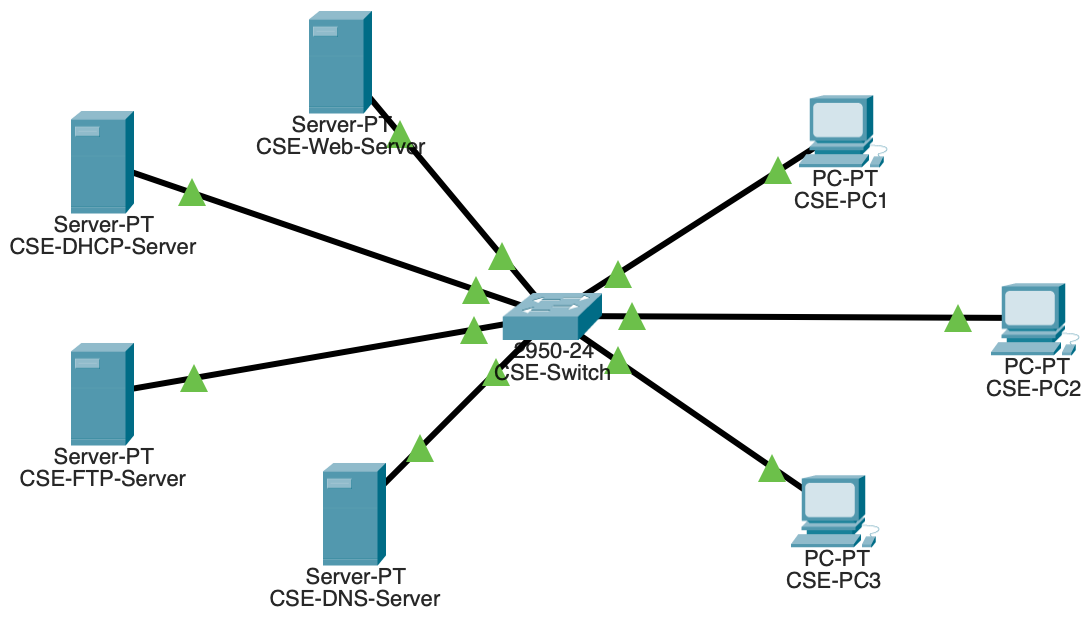
\includegraphics[width=0.75\textwidth]{images/q7_topology.png}
    \caption{Question 7: Complete enterprise CSE LAN topology with 4 dedicated servers.}
    \label{fig:q7_top}
\end{figure}

\begin{figure}[H]
    \centering
    \begin{subfigure}[b]{0.49\textwidth}
        \centering
        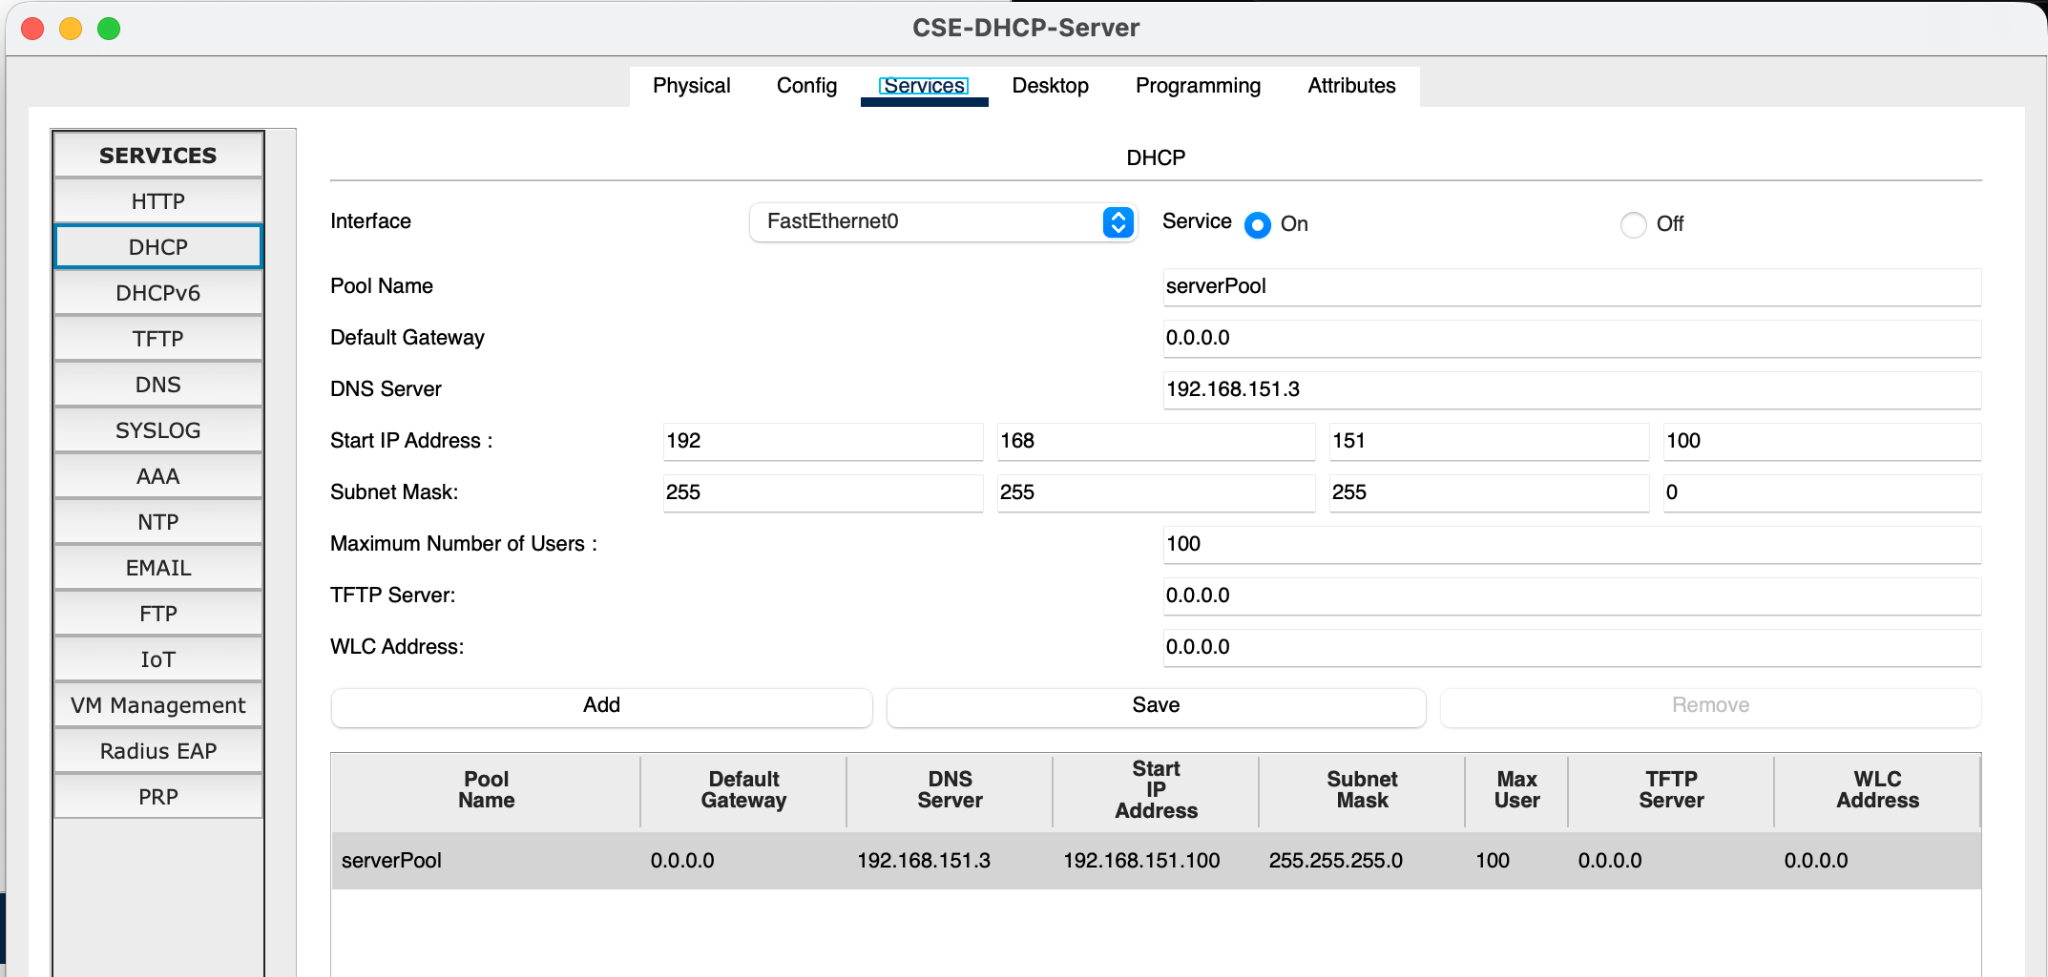
\includegraphics[width=\textwidth]{images/q7_dhcp_server.png}
        \caption{DHCP service pool delivering DNS server pointer.}
        \label{fig:q7_dhcp_srv}
    \end{subfigure}
    \hfill
    \begin{subfigure}[b]{0.49\textwidth}
        \centering
        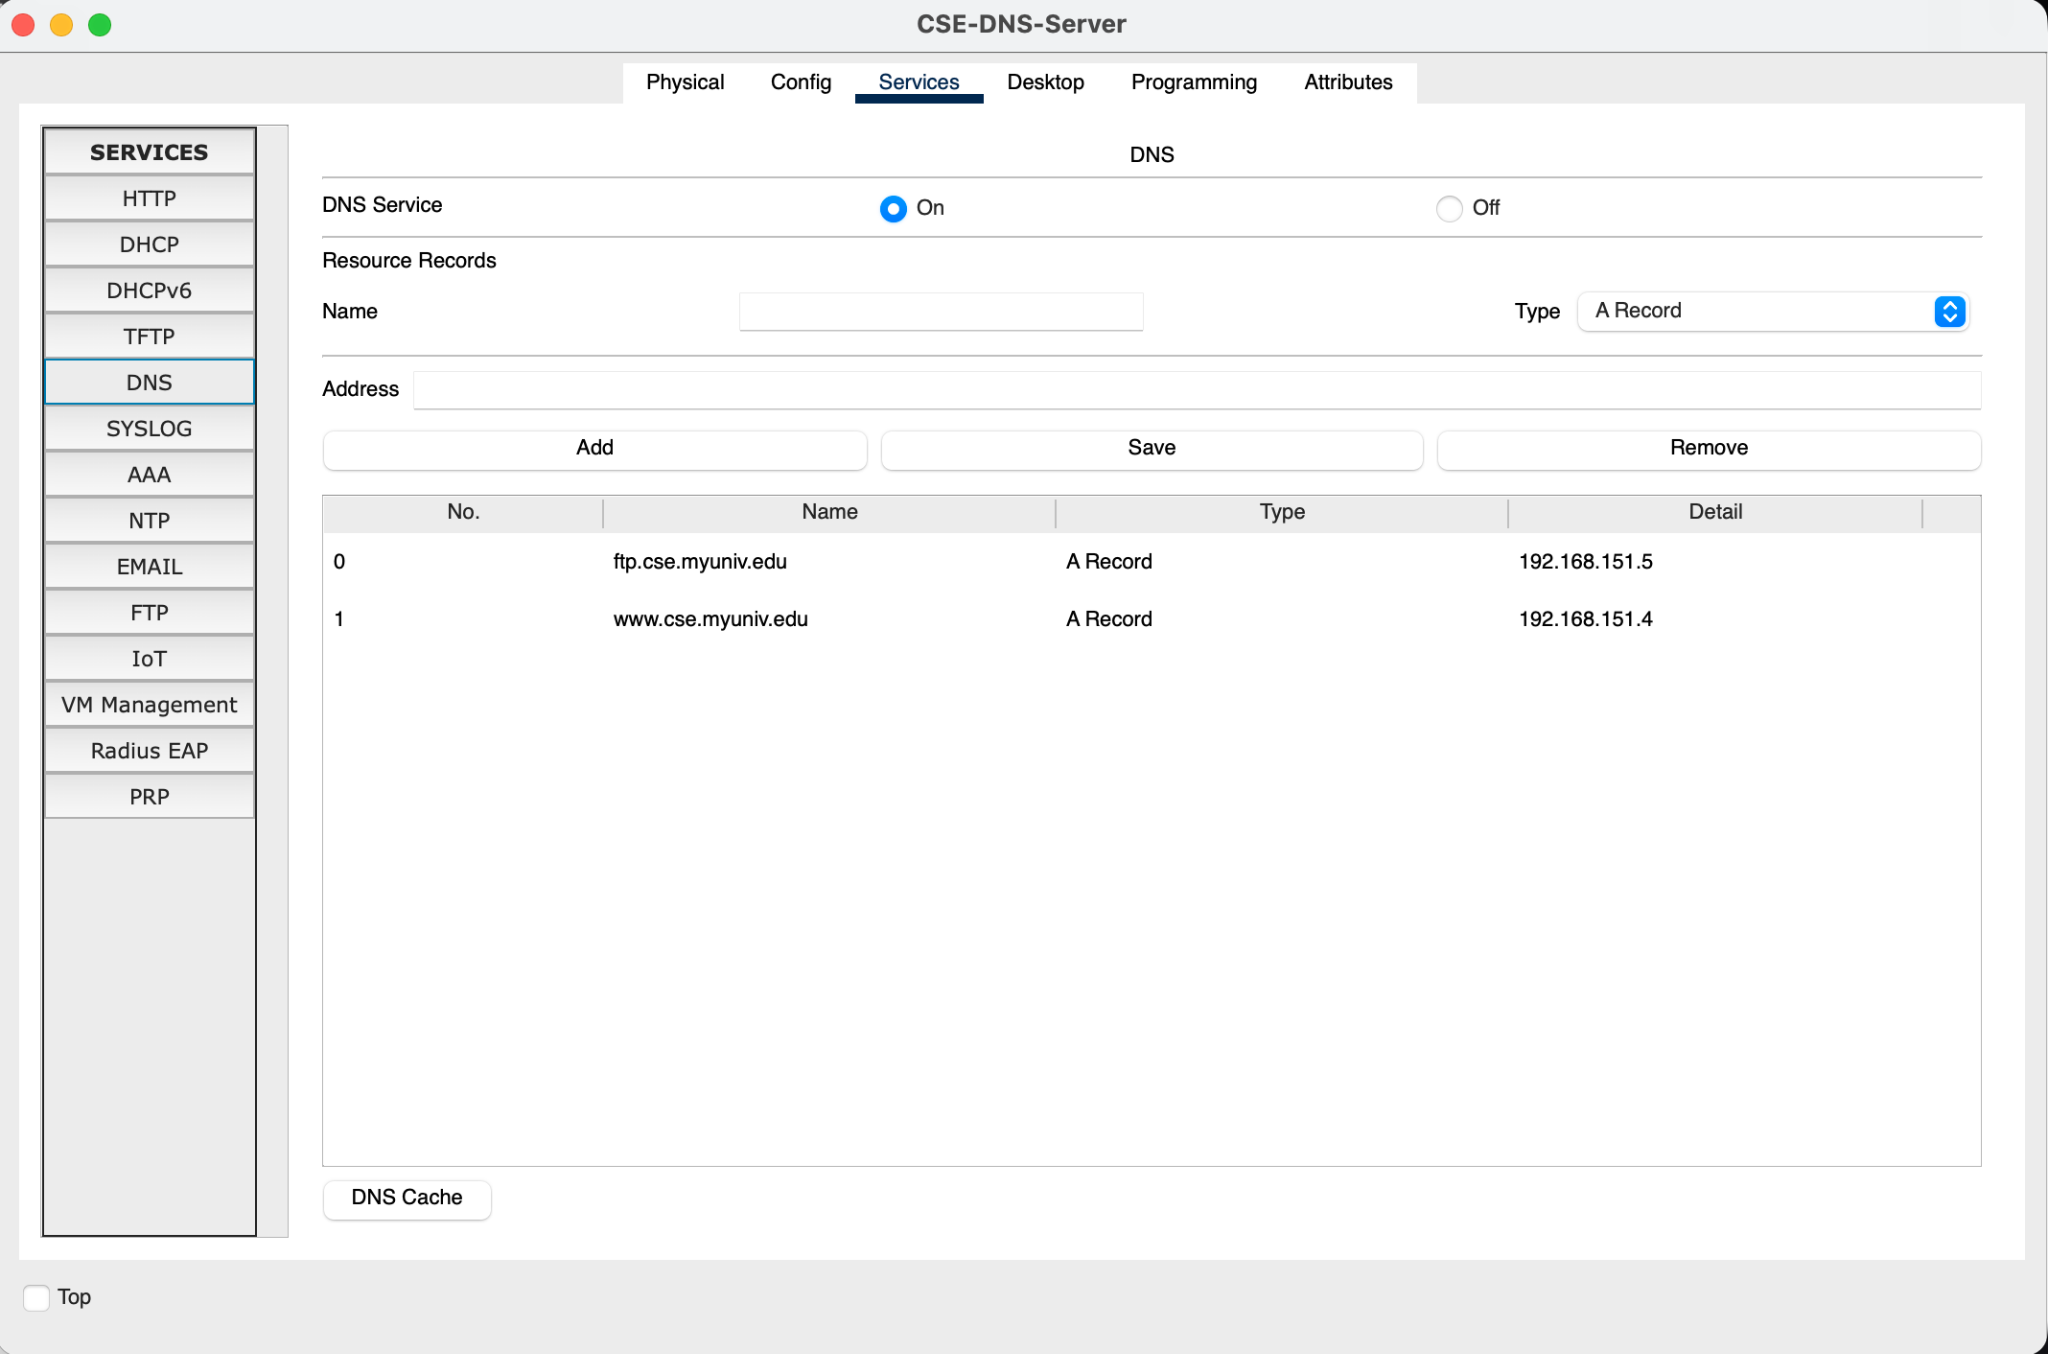
\includegraphics[width=\textwidth]{images/q7_dns_records.png}
        \caption{Authoritative DNS A-records in cse.myuniv.edu.}
        \label{fig:q7_dns_recs}
    \end{subfigure}
    \caption{Question 7: Core network service configurations (DHCP and DNS).}
    \label{fig:q7_infra}
\end{figure}

\newpage

\subsection{Client Dynamic Leasing \& Application Verifications}

\begin{figure}[H]
    \centering
    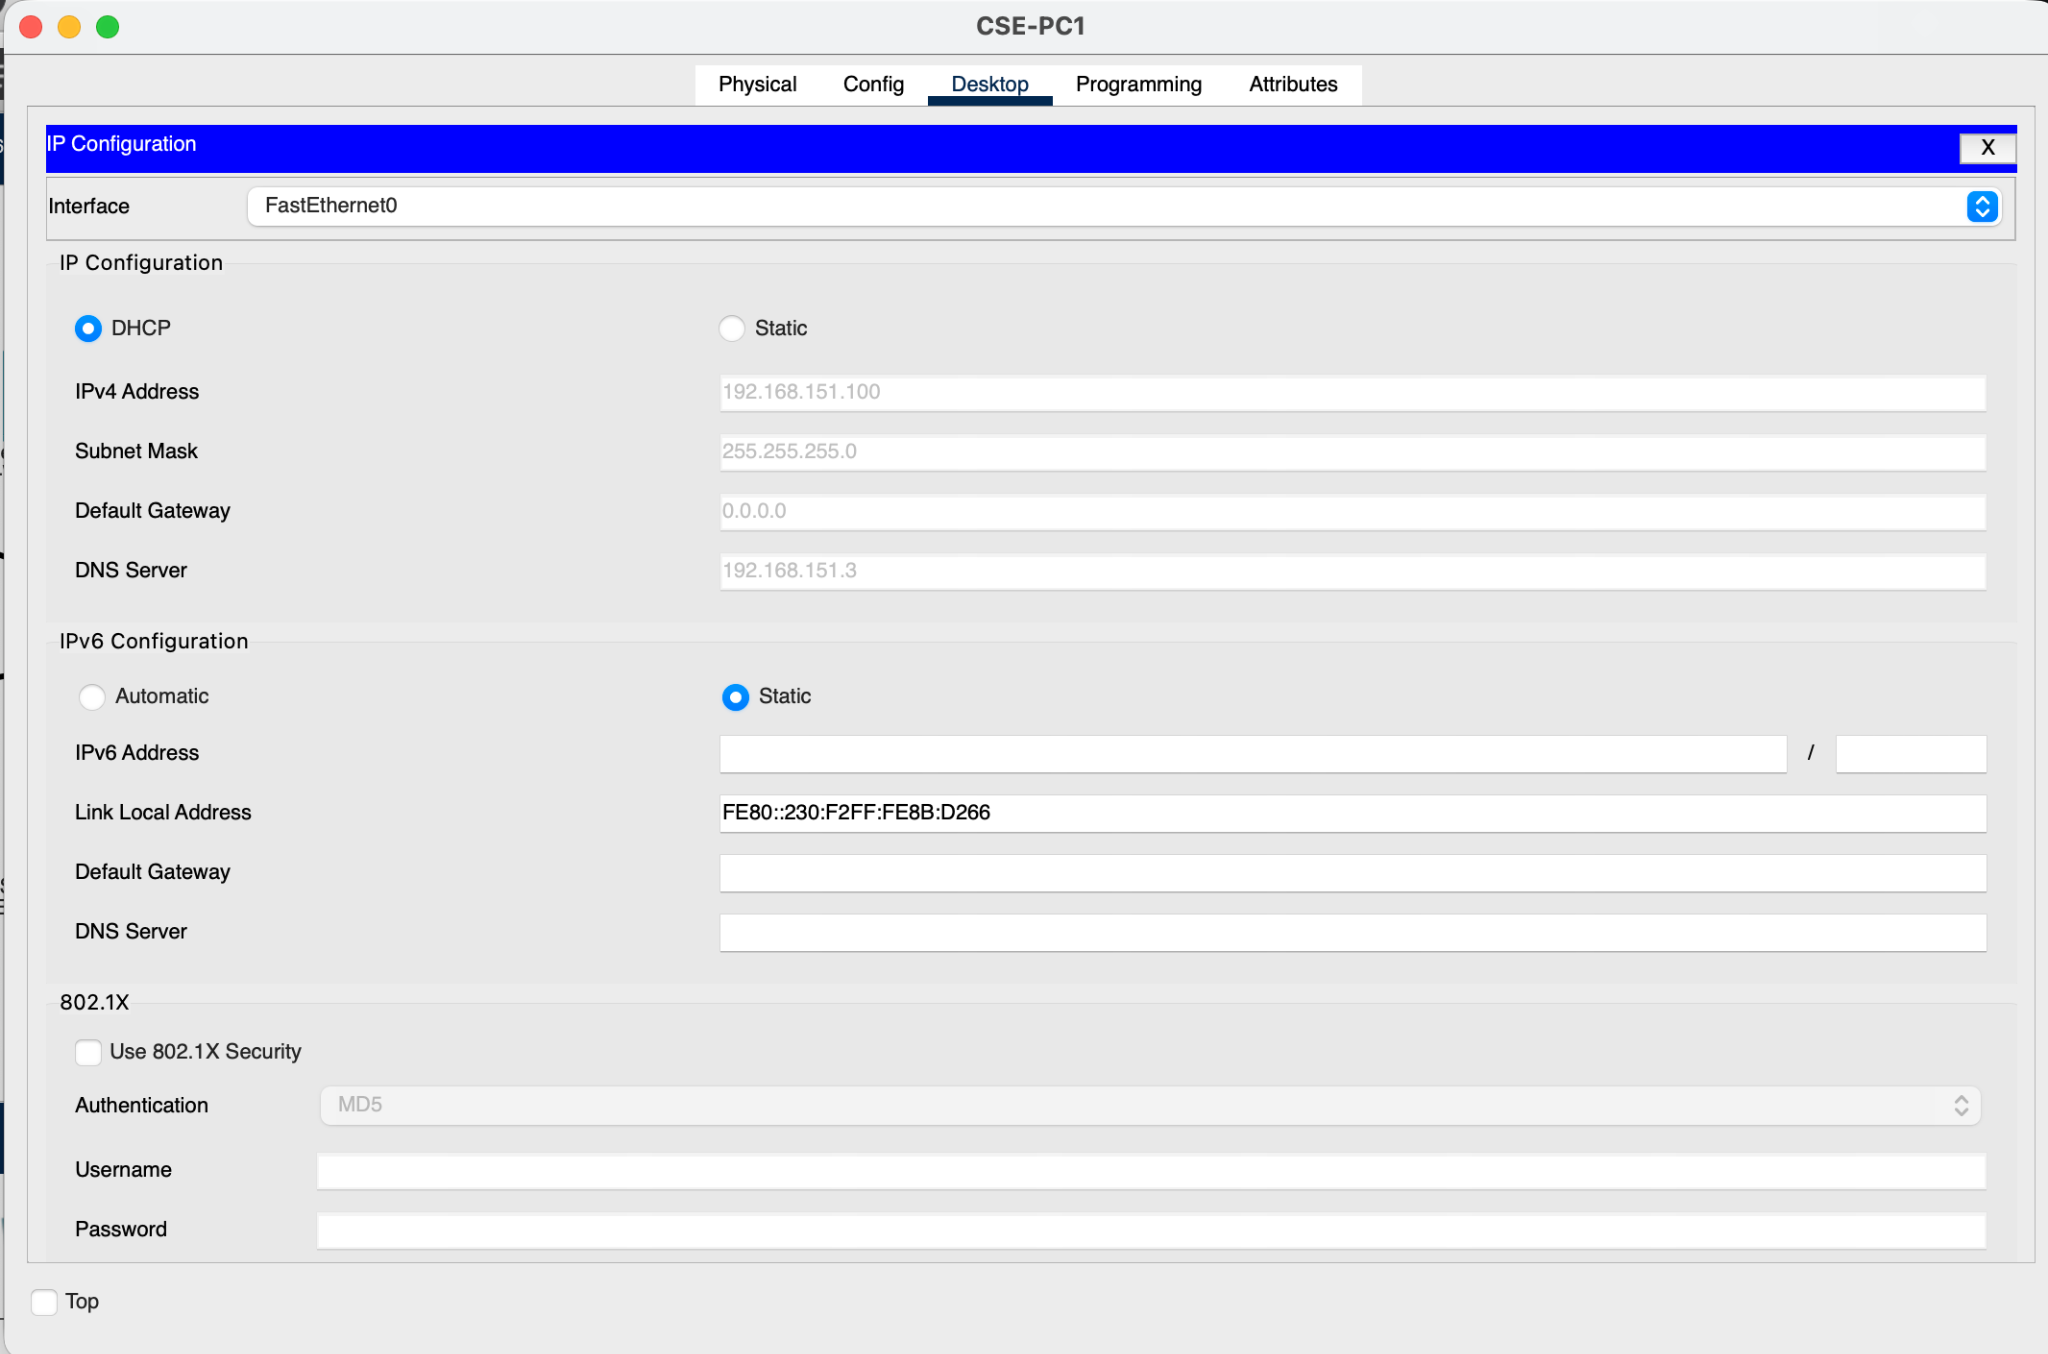
\includegraphics[width=0.80\textwidth]{images/q7_pc_dhcp.png}
    \caption{Question 7: Workstation CSE-PC1 IP configuration showing dynamic IP and DNS server (192.168.151.3).}
    \label{fig:q7_pc_dhcp}
\end{figure}

\begin{figure}[H]
    \centering
    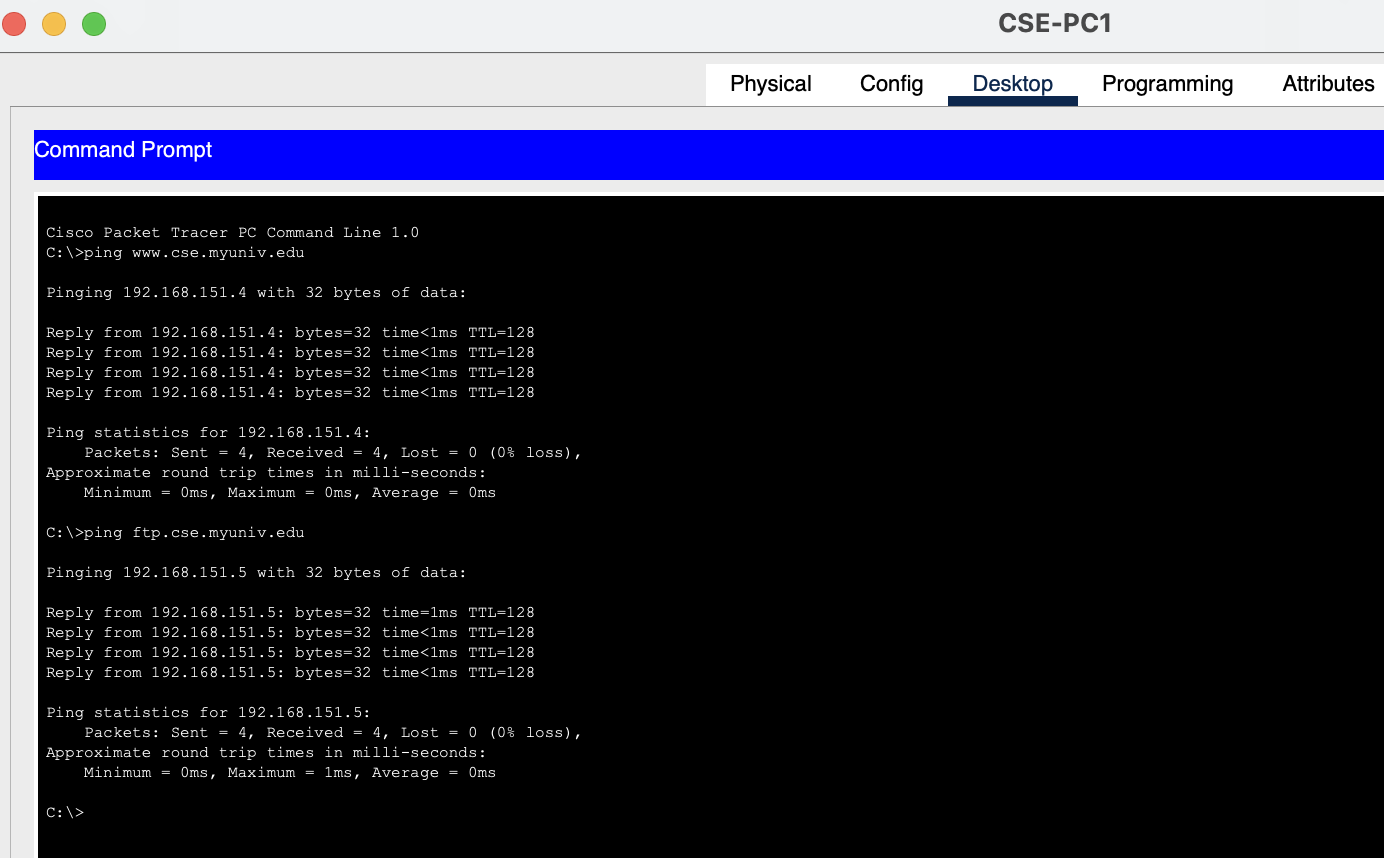
\includegraphics[width=0.82\textwidth]{images/q7_dns_ping.png}
    \caption{Question 7: DNS resolution verification from CSE-PC1 targeting www and ftp domain names.}
    \label{fig:q7_dns_ping}
\end{figure}

\newpage

\begin{figure}[H]
    \centering
    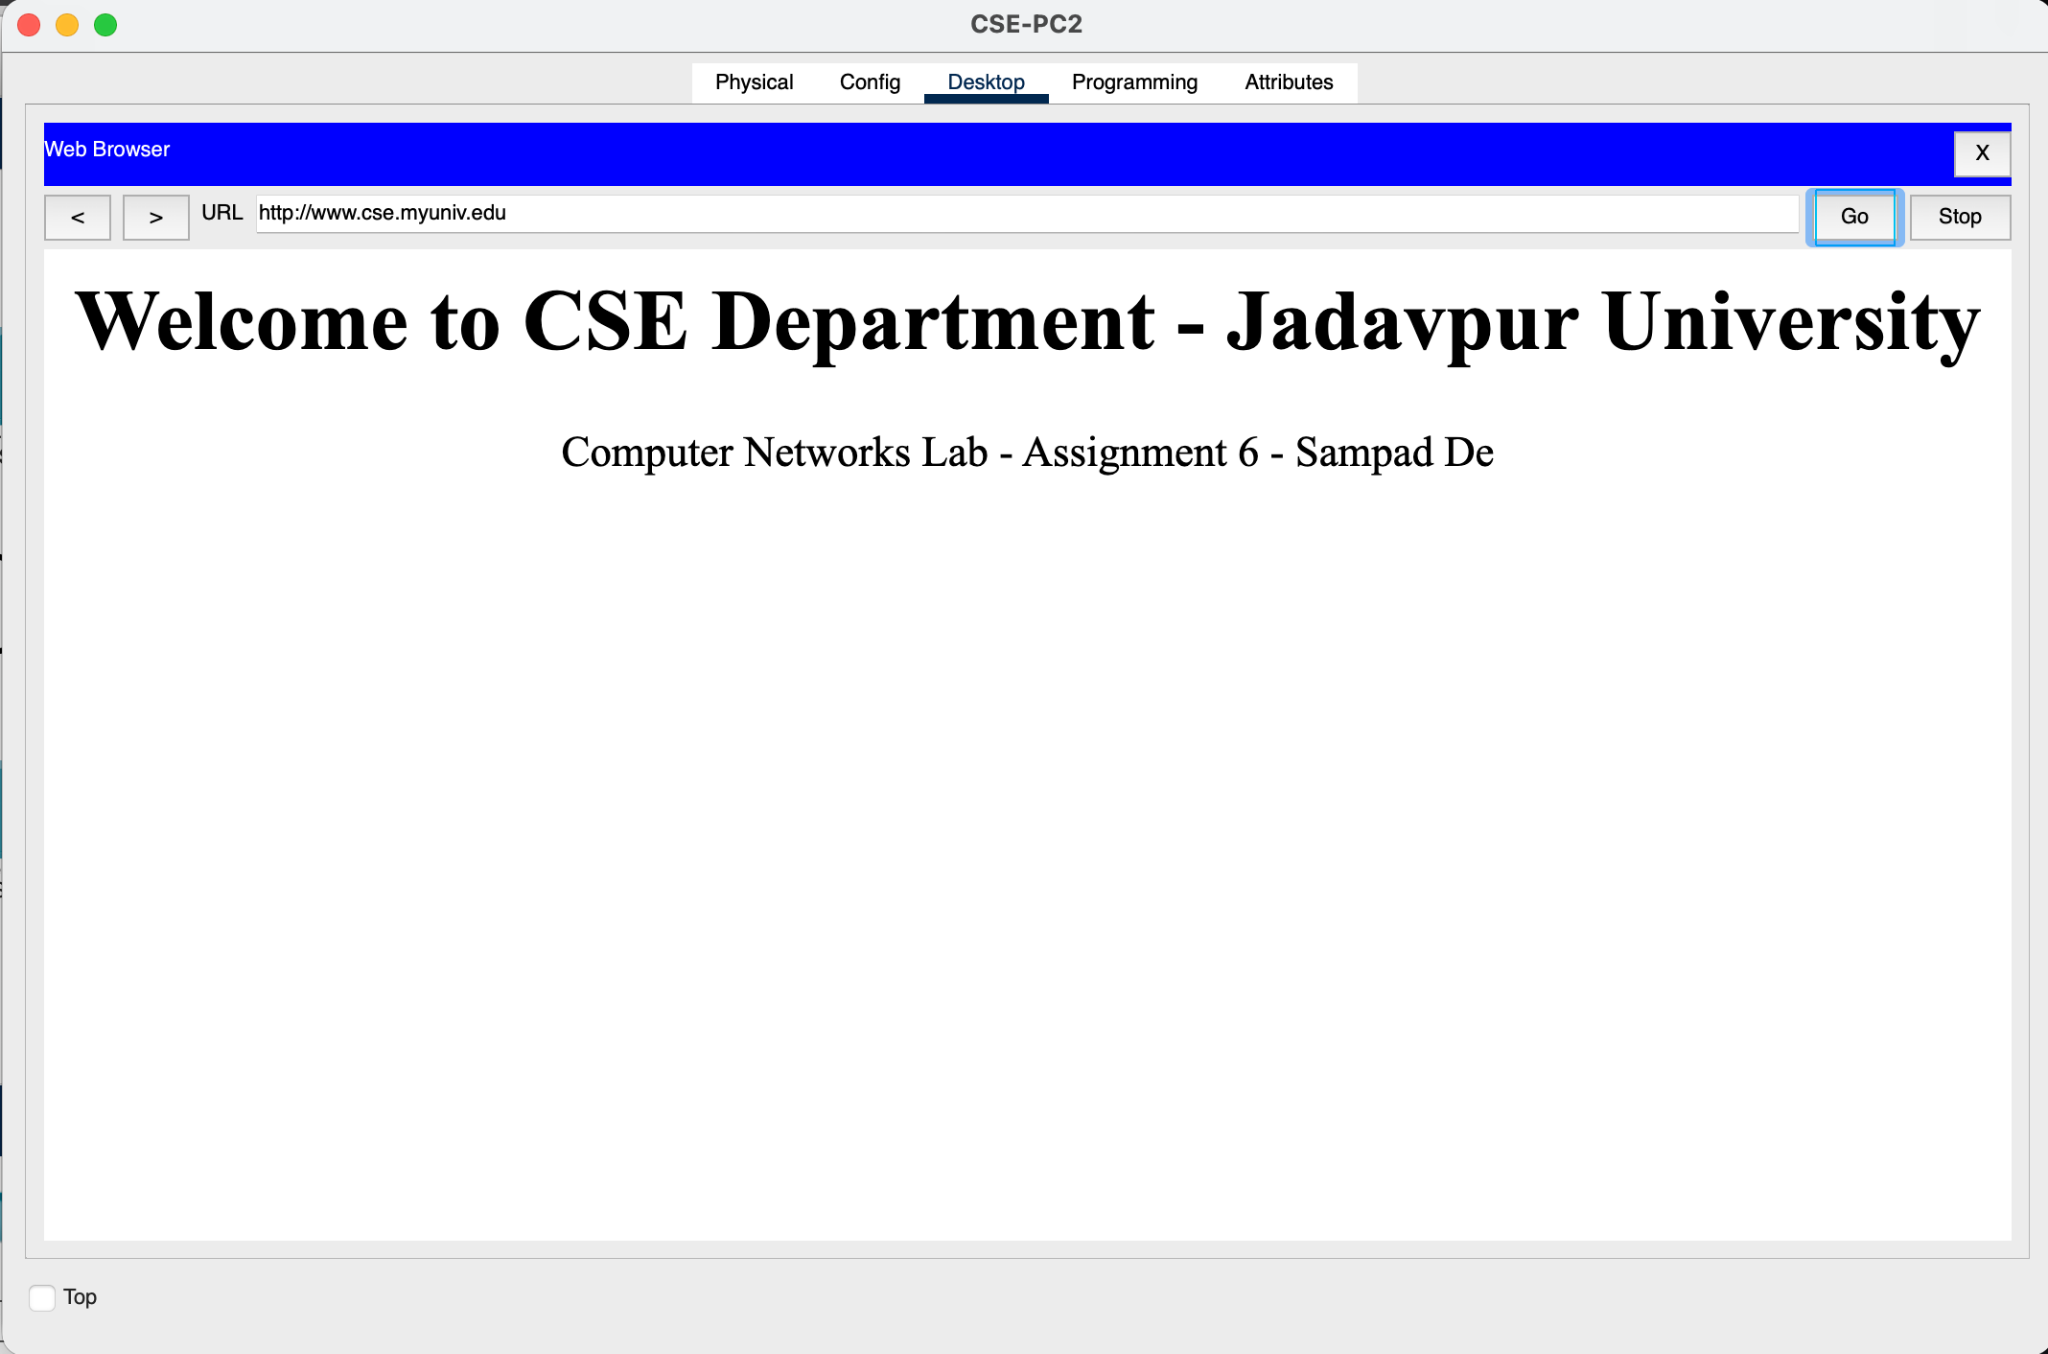
\includegraphics[width=0.90\textwidth]{images/q7_web_browser.png}
    \caption{Question 7: CSE-PC2 web browser rendering custom HTTP landing page for Sampad De.}
    \label{fig:q7_web}
\end{figure}

\begin{figure}[H]
    \centering
    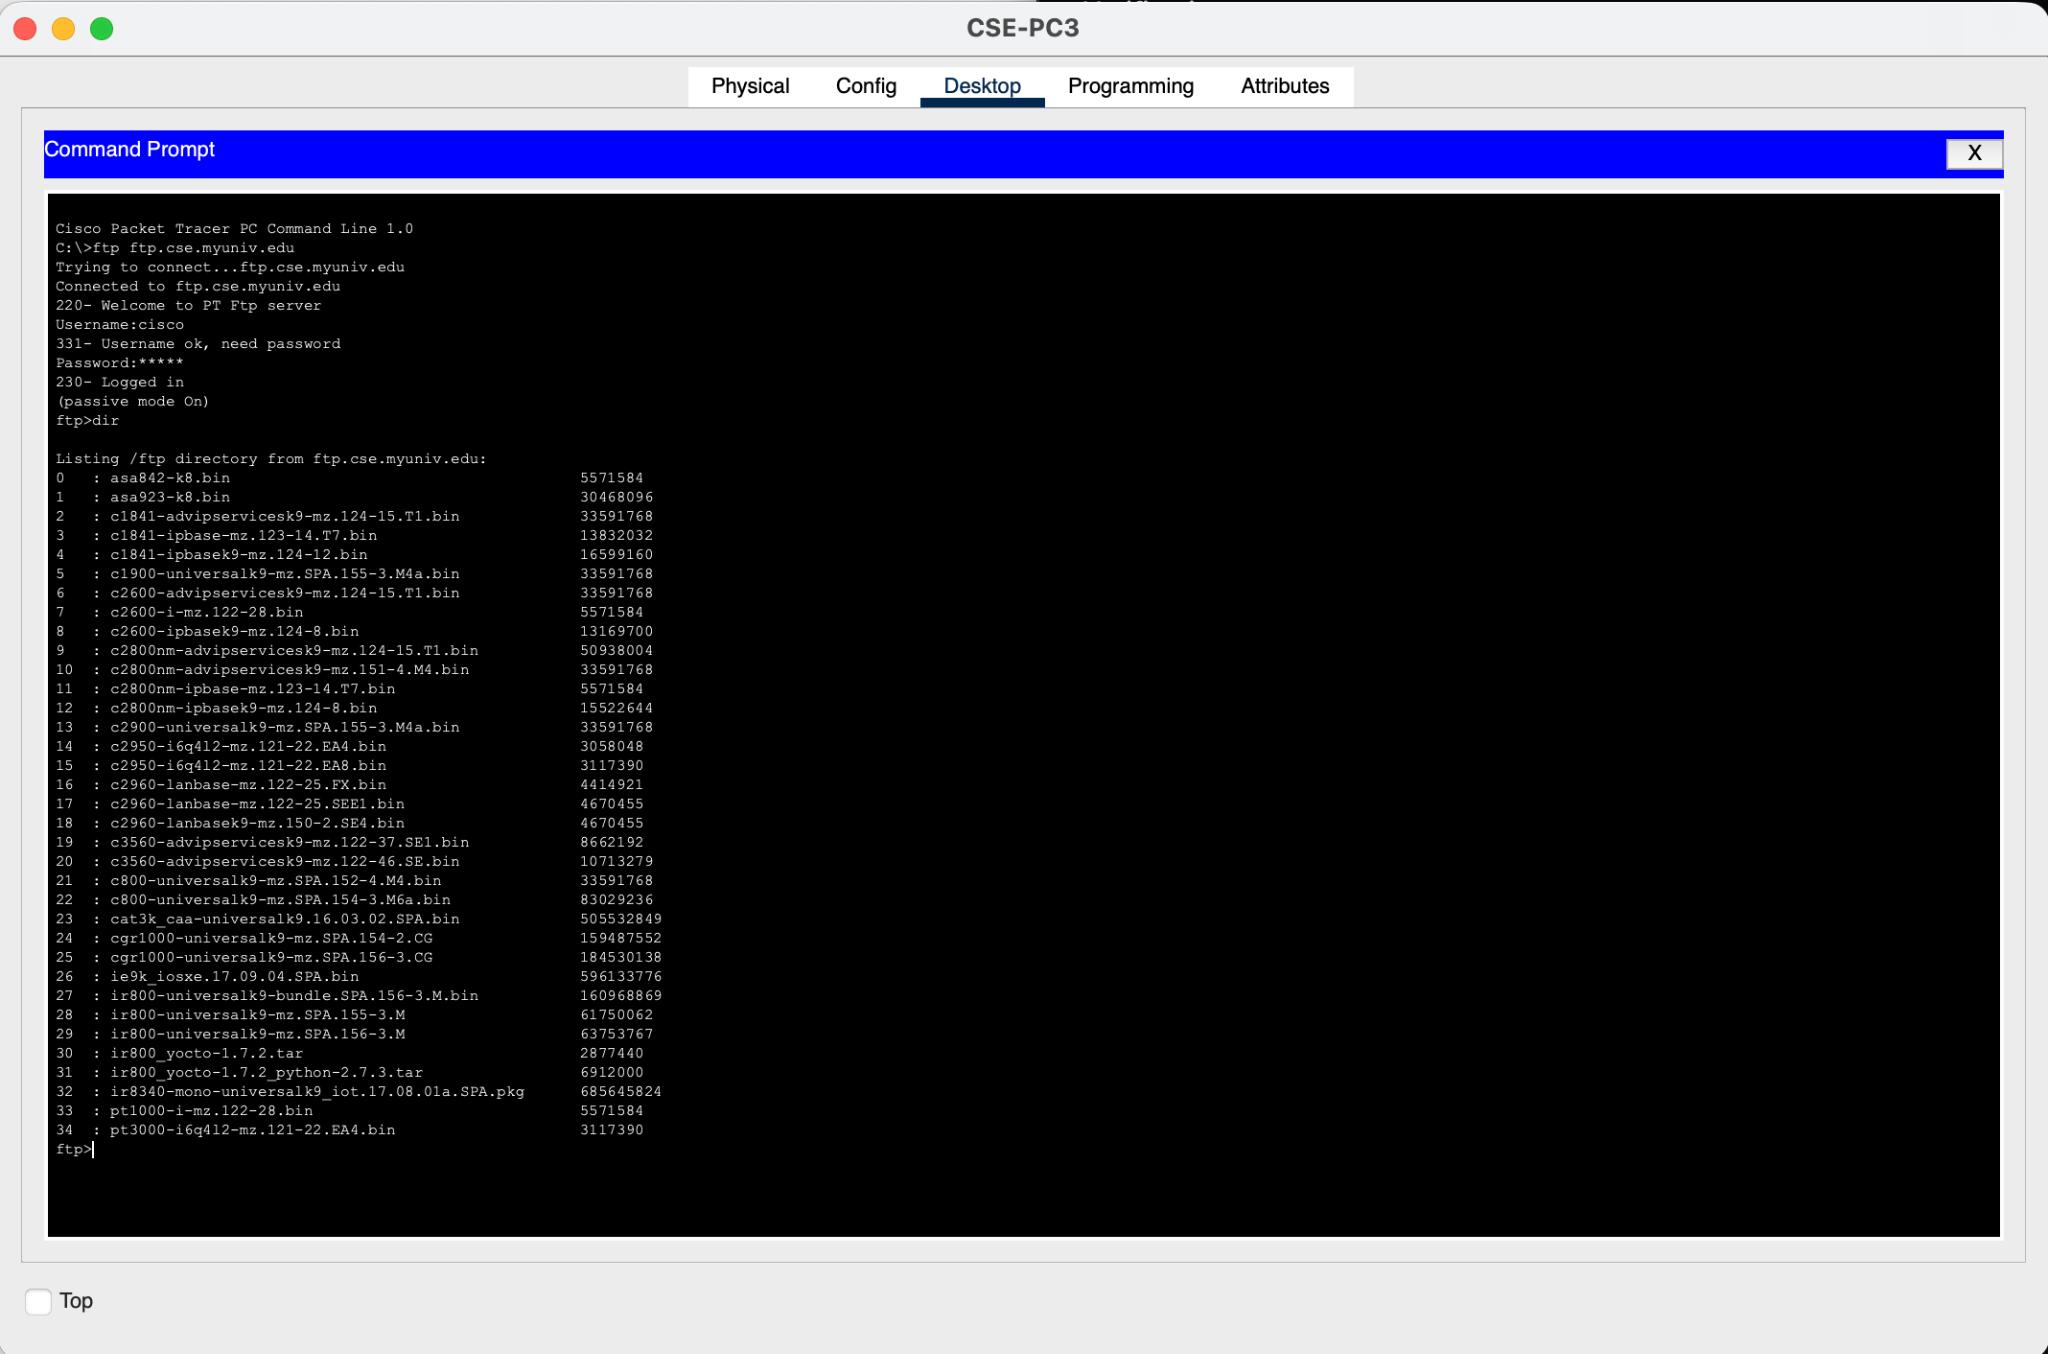
\includegraphics[width=0.90\textwidth]{images/q7_ftp_session.png}
    \caption{Question 7: CSE-PC3 terminal verifying interactive authenticated FTP session and directory listing.}
    \label{fig:q7_ftp}
\end{figure}

\newpage

% ==================== SECTION 9: CONCLUSION ====================
\section{Key Takeaways \& Conclusion}

\begin{enumerate}
    \item \textbf{Physical Media:} Direct host-to-host links (MDI to MDI) require crossover cabling to pair transmit ($TX$) to receive ($RX$) circuitry.
    \item \textbf{Collision Domains:} Hubs blindly repeat bits across a single collision domain, whereas switches micro-segment ports and learn source MAC addresses into CAM tables to enable full-duplex, selective forwarding.
    \item \textbf{ARP Mechanics:} Hosts dynamically map 32-bit IPv4 addresses to 48-bit MAC addresses, initially starting with empty tables and populating upon frame transmission.
    \item \textbf{Subnet Boundaries:} Physical Layer-2 bridging across disparate IP subnets fails without a Layer-3 default gateway to route packets between network IDs.
    \item \textbf{WAN Routing:} Static routing tables (`ip route`) over synchronous serial WAN links enable inter-network routing, accompanied by IPv4 TTL decrementation.
    \item \textbf{Multi-Tier Services:} Automated IP leasing via DHCP (DORA) and hierarchical name resolution via DNS provide the foundation for robust application-layer delivery (HTTP web and FTP storage).
\end{enumerate}

% ==================== SECTION 10: REFERENCES ====================
\section{References}
\begin{enumerate}[leftmargin=*]
    \item \textbf{Project Source Code Repository:} \url{https://github.com/Sampad2006/CN-Lab-Assignments}.
    \item \textbf{AI Assistance :} AI (Gemini 3.8 Flash) was utilized to generate latex chart configurations and also to use Cisco Packet Tracer. All specific setups,screenshots and answers I have done myself .
\end{enumerate}

\end{document}
